\documentclass[aspectratio=169,10pt,fontset=fandol]{ctexbeamer}
\usepackage{amsmath,amssymb,mathtools,bm,mathrsfs}
\usepackage{graphicx,booktabs,array,tabularx,multirow}
\usepackage{tikz,pgfplots,xparse,xstring,mdframed}
\usetikzlibrary{arrows.meta,calc,angles,positioning,shapes.geometric,graphs}
\pgfplotsset{compat=1.18}
\usetheme{fduclassroom}
\setbeamerfont{normal text}{size=\normalsize}
\setbeamerfont{title}{size=\large}
\setbeamerfont{subtitle}{size=\normalsize}
\setbeamerfont{frametitle}{size=\large}
\setbeamerfont{framesubtitle}{size=\small}
\setbeamerfont{block title}{size=\normalsize}
\setbeamerfont{block body}{size=\normalsize}
\setbeamerfont{section in toc}{size=\normalsize}
\setbeamerfont{section in head/foot}{size=\footnotesize}
\setbeamerfont{author in head/foot}{size=\footnotesize}
\setbeamerfont{title in head/foot}{size=\footnotesize}
\setbeamerfont{date in head/foot}{size=\footnotesize}
\setbeamertemplate{navigation symbols}{}
\setbeamertemplate{itemize item}{\normalsize\textbullet}
\setbeamertemplate{itemize subitem}{\small\textbullet}
\setbeamercolor{structure}{fg=blue!65!black}
\setbeamercolor{block title}{fg=blue!65!black,bg=blue!8}
\setbeamercolor{block body}{fg=black,bg=blue!3}

% ctex fontset=fandol; system fonts are not redistributed.

\mdfdefinestyle{extrastyle}{%
    linecolor=gray,
    linewidth=0.8pt,
    frametitlerule=true,
    frametitlebackgroundcolor=gray!10,
    backgroundcolor=gray!5,
    skipabove=10pt,
    skipbelow=10pt,
    innertopmargin=6pt,
    innerbottommargin=6pt
}
\newenvironment{extra}{\begin{mdframed}[style=extrastyle, frametitle={* 选读内容（不要求掌握）}]}{\end{mdframed}}
\newenvironment{custom}[1]{\par\noindent\textbf{#1}\quad}{\par\vspace{0.8em}}
\newenvironment{idea}{\par\noindent\textbf{思路}\quad}{\par\vspace{0.4em}}
\newenvironment{warning}{\par\noindent\textbf{注：}\quad}{\par\vspace{0.8em}}
\newenvironment{intuition}{\par\noindent\textbf{直观理解}\quad}{\par\vspace{0.8em}}
\NewDocumentEnvironment{application}{O{}}
{\par\noindent\textbf{应用拓展\IfStrEq{#1}{}{}{——#1}}\quad}
{\par\vspace{0.8em}}
\newcommand{\dd}{\mathrm{d}}
\newcommand{\ee}{\mathrm{e}}
\newcommand{\ii}{\mathrm{i}}
\newcommand{\RR}{\mathbb{R}}
\newcommand{\upcite}[1]{\textsuperscript{\textsuperscript{\cite{#1}}}}
\DeclareMathOperator*{\argmax}{\mathrm{arg\,max}}
\DeclareMathOperator*{\argmin}{\mathrm{arg\,min}}
\title{第一章}
\begin{document}
\section{数学内容}
% FRAME-ID F001
\begin{frame}[t,fragile]{目录（1/2）}
\normalsize
{\color{blue}\normalsize 1. 数学内容\par}\vspace{0.3em}
{\color{gray!40}\normalsize 2. 数列的一般定义\par}\vspace{0.3em}
{\color{gray!40}\normalsize 3. 拓展阅读：数列的应用\par}\vspace{0.3em}
{\color{gray!40}\normalsize 4. 差分及其应用\par}\vspace{0.3em}
{\color{gray!40}\normalsize 5. 从实数的完备性说起\par}\vspace{0.3em}
{\color{gray!40}\normalsize 6. 实数的完备性简介\par}\vspace{0.3em}
{\color{gray!40}\normalsize 7. 数列极限\par}\vspace{0.3em}
{\color{gray!40}\normalsize 8. 收敛数列的基本性质\par}\vspace{0.3em}
{\color{gray!40}\normalsize 9. 极限存在性定理\par}\vspace{0.3em}
{\color{gray!40}\normalsize 10. 拓展阅读：Landau 符号-小o与大O\par}\vspace{0.3em}
\end{frame}
% FRAME-ID F002
\begin{frame}[t,fragile]{目录（2/2）}
\normalsize
{\color{gray!40}\normalsize 11. 第2章课后习题\par}\vspace{0.3em}
{\color{gray!40}\normalsize 12. 第2章参考答案与提示\par}\vspace{0.3em}
\end{frame}
% FRAME-ID F003
\begin{frame}[t,fragile]{数学内容}
\footnotesize
{\footnotesize
% SOURCE-BEGIN U0001 0 33

\maketitle
\vspace{-1em}



% SOURCE-END U0001
}
\end{frame}
\section{数列的一般定义}
% FRAME-ID F004
\begin{frame}[t,fragile]{目录（1/2）}
\normalsize
{\color{black}\normalsize 1. 数学内容\par}\vspace{0.3em}
{\color{blue}\normalsize 2. 数列的一般定义\par}\vspace{0.3em}
{\color{gray!40}\normalsize 3. 拓展阅读：数列的应用\par}\vspace{0.3em}
{\color{gray!40}\normalsize 4. 差分及其应用\par}\vspace{0.3em}
{\color{gray!40}\normalsize 5. 从实数的完备性说起\par}\vspace{0.3em}
{\color{gray!40}\normalsize 6. 实数的完备性简介\par}\vspace{0.3em}
{\color{gray!40}\normalsize 7. 数列极限\par}\vspace{0.3em}
{\color{gray!40}\normalsize 8. 收敛数列的基本性质\par}\vspace{0.3em}
{\color{gray!40}\normalsize 9. 极限存在性定理\par}\vspace{0.3em}
{\color{gray!40}\normalsize 10. 拓展阅读：Landau 符号-小o与大O\par}\vspace{0.3em}
\end{frame}
% FRAME-ID F005
\begin{frame}[t,fragile]{目录（2/2）}
\normalsize
{\color{gray!40}\normalsize 11. 第2章课后习题\par}\vspace{0.3em}
{\color{gray!40}\normalsize 12. 第2章参考答案与提示\par}\vspace{0.3em}
\end{frame}
% FRAME-ID F006
\begin{frame}[t,fragile]{数列的一般定义}
\footnotesize
{\footnotesize
% SOURCE-BEGIN U0002 0 97


数列是以正整数集为定义域的特殊函数，用以刻画有序离散数量变化。作为初等与高等数学的过渡概念，它提供了理解无穷、极限的直观载体，能够有效建模分期、迭代、时序等现实问题。





% SOURCE-END U0002
}
\end{frame}
% FRAME-ID F007
\begin{frame}[t,fragile]{数列的一般定义}
\footnotesize
\begin{block}{定义}
{\footnotesize
% SOURCE-BEGIN U0003 0 377

无穷多个数按下列顺序排列：

$$
a_1, a_2, \cdots, a_n, \cdots
$$

称为数列，记为 $\left\{a_n\right\}$ ,其中 $a_n$ 称为数列的通项或一般项；正整数 $n$ 称为 $a_n$ 的下标。

数列也可以看作定义在正整数集 $\mathbb{N}^+=\{1,2,3,\cdots\}$ 上、取实数值的函数。因此，数列既有函数的本质，又有离散变量的特点。 函数 $y=f(x)$ 的自变量可以在区间中连续取值，而数列只在 $n=1,2,\ldots$ 这些正整数处取值。 因此，数列可以看作一种特殊函数：
\[
a_n=f(n),\qquad n\in\mathbb{N}^+.
\]
讨论数列时，项的顺序不可随意改变；同一组数字若排列顺序不同，通常就是不同数列。

% SOURCE-END U0003
}
\end{block}
\end{frame}
% FRAME-ID F008
\begin{frame}[t,fragile]{数列的一般定义}
\footnotesize
{\footnotesize
% SOURCE-BEGIN U0004 0 657
\begin{custom}{由递推关系表示数列}
	
	$k$阶递推的含义是将数列自第$k+1$项起的每一项由前k项表示：
	
	\begin{equation*}
		\begin{cases}
			a_1 = c_1, \\
			a_2 = c_2, \\
			\quad \vdots \\
			a_k = c_k, \\
			a_n = f(a_{n-1}, a_{n-2}, \dots, a_{n-k}), & \forall n > k, \; n \in \mathbb{N}^*
		\end{cases}
	\end{equation*}
	例如：
	
	一阶递推：
	\begin{equation*}
		\begin{cases}
			a_1 = 1, \\
			a_n = 2 a_{n-1} + 3, & (n \ge 2, \; n \in \mathbb{N}^+)
		\end{cases}
	\end{equation*}
	
	二阶递推：
	\[
	a_1 = 1,\ a_2 = 1,\ a_n = a_{n-1} + a_{n-2}\ (n \geq 3),
	\]
	这就是著名的\textbf{斐波那契数列}：\(1,1,2,3,5,8,13,21,\dots\)
	
	斐波那契数列既来自兔子繁殖等理想化模型，也常出现在向日葵花盘、松果鳞片等植物的螺旋计数中。
\end{custom}
% SOURCE-END U0004
}
\end{frame}
% FRAME-ID F009
\begin{frame}[t,fragile]{数列的一般定义}
\footnotesize
\begin{block}{例题}
{\footnotesize
% SOURCE-BEGIN U0005 0 122
判断下列对象能否确定一个数列，并说明理由。
\[
(1)\ a_n=\frac{n+1}{2n-1};\qquad
(2)\ a_1=1,\ a_{n+1}=2a_n+1;\qquad
(3)\ 1,2,4,\ldots .
\]

% SOURCE-END U0005
}
\end{block}
\pause
{\footnotesize
\textbf{解：}
% SOURCE-BEGIN U0006 0 263
(1) 给出了通项公式，对每个正整数 $n$ 都能唯一确定 $a_n$，因此确定一个数列。

(2) 给出了初值和递推关系。 由 $a_1=1$ 可依次得到
\[
a_2=3,\quad a_3=7,\quad a_4=15,\ldots
\]
因此也确定一个数列。

(3) 只列出前三项，不能唯一确定一个数列。 例如 $a_n=2^{n-1}$ 的前三项为 $1,2,4$；但 $b_1=1,b_2=2,b_3=4,b_n=0(n\ge4)$ 也有同样前三项。 因此仅凭有限项通常不能严格确定无穷数列。

% SOURCE-END U0006
}
\end{frame}
% FRAME-ID F010
\begin{frame}[t,fragile]{数列的一般定义}
\footnotesize
\begin{block}{例题}
{\footnotesize
% SOURCE-BEGIN U0007 0 137
设某药物每隔固定时间给药一次，每次给药后体内新增浓度 $C_0$，两次给药之间保留比例为 $q$，其中 $0<q<1$。 若 $A_n$ 表示第 $n$ 次给药后体内药物浓度，则可建立递推模型
\[
A_{n+1}=qA_n+C_0.
\]
求该模型的稳定浓度。

% SOURCE-END U0007
}
\end{block}
\end{frame}
% FRAME-ID F011
\begin{frame}[t,fragile]{数列的一般定义}
\footnotesize
{\footnotesize
\textbf{解：}
% SOURCE-BEGIN U0008 0 298
若 $A_n$ 收敛到稳定浓度 $A$，则在极限状态下应满足
\[
A=qA+C_0.
\]
解得
\[
A=\frac{C_0}{1-q}.
\]
为了说明这一步不是形式猜测，令 $B_n=A_n-A$。 由 $A=qA+C_0$ 及 $A_{n+1}=qA_n+C_0$ 得
\[
B_{n+1}=A_{n+1}-A=q(A_n-A)=qB_n.
\]
因此
\[
B_n=q^{n-1}B_1.
\]
由于 $0<q<1$，有 $q^{n-1}\to0$，所以 $B_n\to0$，即
\[
A_n\to A=\frac{C_0}{1-q}.
\]

% SOURCE-END U0008
}
\end{frame}
% FRAME-ID F012
\begin{frame}[t,fragile]{数列的一般定义}
\footnotesize
{\footnotesize
% SOURCE-BEGIN U0009 0 92
本例先使用高中阶段熟悉的等比数列极限 $q^n\to0\ (0<q<1)$ 来说明递推模型的稳定状态。本章后半部分将用 $\varepsilon$--$N$ 语言严格定义数列收敛。

% SOURCE-END U0009
}
\end{frame}
\section{拓展阅读：数列的应用}
% FRAME-ID F013
\begin{frame}[t,fragile]{目录（1/2）}
\normalsize
{\color{black}\normalsize 1. 数学内容\par}\vspace{0.3em}
{\color{black}\normalsize 2. 数列的一般定义\par}\vspace{0.3em}
{\color{blue}\normalsize 3. 拓展阅读：数列的应用\par}\vspace{0.3em}
{\color{gray!40}\normalsize 4. 差分及其应用\par}\vspace{0.3em}
{\color{gray!40}\normalsize 5. 从实数的完备性说起\par}\vspace{0.3em}
{\color{gray!40}\normalsize 6. 实数的完备性简介\par}\vspace{0.3em}
{\color{gray!40}\normalsize 7. 数列极限\par}\vspace{0.3em}
{\color{gray!40}\normalsize 8. 收敛数列的基本性质\par}\vspace{0.3em}
{\color{gray!40}\normalsize 9. 极限存在性定理\par}\vspace{0.3em}
{\color{gray!40}\normalsize 10. 拓展阅读：Landau 符号-小o与大O\par}\vspace{0.3em}
\end{frame}
% FRAME-ID F014
\begin{frame}[t,fragile]{目录（2/2）}
\normalsize
{\color{gray!40}\normalsize 11. 第2章课后习题\par}\vspace{0.3em}
{\color{gray!40}\normalsize 12. 第2章参考答案与提示\par}\vspace{0.3em}
\end{frame}
% FRAME-ID F015
\begin{frame}[t,fragile]{拓展阅读：数列的应用}
\footnotesize
{\footnotesize
% SOURCE-BEGIN U0010 0 140


数列不仅仅是课本上的抽象概念，它在我们的日常生活和现代生产中有着广泛的应用。下面介绍几个有趣的实例。

\textbf{算法分析与计算机科学}

在计算机科学中，算法的\textbf{时间复杂度}经常用数列来描述。例如，考虑一个在有序数组中查找元素的算法：


% SOURCE-END U0010
}
\end{frame}
% FRAME-ID F016
\begin{frame}[t,fragile]{拓展阅读：数列的应用}
\footnotesize
{\footnotesize
% SOURCE-BEGIN U0011 0 497
\begin{itemize}
\item \textbf{二分查找}：每次将搜索范围缩小一半。在最坏情况下，需要查找的次数满足递推关系：
\[
T(n) = T\left(\dfrac{n}{2}\right) + 1,\quad T(1) = 1\qquad(n=2^m).
\]
解这个递推，得到 \(T(n)=\log_2 n+1\)。对一般的数组长度，最坏查找次数随 $n$ 按对数级增长，常记为 \(O(\log n)\)。这里先把 \(O(\log n)\) 理解为“增长量级不超过对数函数的常数倍”，Landau 大 \(O\) 记号将在第 3.10 节正式定义。


一个著名的例子是\textbf{汉诺塔}问题：把 \(n\) 个圆盘从一根柱子移到另一根，最少需要移动的次数满足：
\[
H_n = 2H_{n-1} + 1,\quad H_1 = 1.
\]
解这个递推得 \(H_n = 2^n - 1\)——指数增长！64 个圆盘需要移动 \(2^{64}-1\) 次，即使每秒移动一次，也需要约 5849 亿年。
\end{itemize}
% SOURCE-END U0011
}
\end{frame}
% FRAME-ID F017
\begin{frame}[t,fragile]{拓展阅读：数列的应用}
\footnotesize
{\footnotesize
% SOURCE-BEGIN U0012 0 100


\textbf{自然界中的斐波那契数列}

斐波那契数列 \(1, 1, 2, 3, 5, 8, 13, 21, 34, 55, \ldots\) 在一些植物结构的计数中经常出现：


% SOURCE-END U0012
}
\end{frame}
% FRAME-ID F018
\begin{frame}[t,fragile]{拓展阅读：数列的应用}
\footnotesize
{\footnotesize
% SOURCE-BEGIN U0013 0 410
\begin{itemize}
\item \textbf{向日葵的花盘}：种子排列成两组螺旋线，一组顺时针，一组逆时针，数量通常是相邻的斐波那契数（如 34 和 55，或 55 和 89）。
\item \textbf{松果的鳞片}：排列也呈现斐波那契螺旋。
\item \textbf{螺壳的形状}：许多螺壳可近似为对数螺线，但通常不能据此断言它们是黄金螺线或满足斐波那契比例。黄金分割与斐波那契数列之间的严格联系是 \(\lim\limits_{n \to \infty} \dfrac{F_{n+1}}{F_n}=\varphi\)。
\item \textbf{蜜蜂的家族树}：雄蜂（由未受精卵发育而来）的祖先数量构成斐波那契数列。
\item \textbf{花瓣数}：许多花的花瓣数是 3（百合）、5（飞燕草）、8（翠雀）、13（金盏花）、21（紫菀）等斐波那契数。
\end{itemize}
% SOURCE-END U0013
}
\end{frame}
% FRAME-ID F019
\begin{frame}[t,fragile]{拓展阅读：数列的应用}
\footnotesize
{\footnotesize
% SOURCE-BEGIN U0014 0 283
\begin{center}
\begin{tikzpicture}
% 简单的向日葵螺旋示意图
\foreach \i in {1,...,50} {
    \pgfmathsetmacro{\r}{0.3*sqrt(\i)}
    \pgfmathsetmacro{\theta}{137.5*\i}
    \filldraw[orange] (\theta:\r) circle (1.5pt);
}
\node at (0, -3) {向日葵种子的螺旋排列（示意图）};
\end{tikzpicture}
\end{center}
% SOURCE-END U0014
}
\end{frame}
% FRAME-ID F020
\begin{frame}[t,fragile]{拓展阅读：数列的应用}
\footnotesize
{\footnotesize
% SOURCE-BEGIN U0015 0 166


这类计数与植物生长点的旋转角、局部拥挤和空间利用有关。具体数目会随物种与个体变化，因此应把它们理解为常见模式，而不是没有例外的自然定律。


\textbf{工程中的递归设计与分形}

在工程和建筑设计领域，许多结构采用\textbf{自相似}的设计——即整体与局部形状相似。这种递归结构可以用数列来描述。


% SOURCE-END U0015
}
\end{frame}
% FRAME-ID F021
\begin{frame}[t,fragile]{拓展阅读：数列的应用}
\footnotesize
{\footnotesize
% SOURCE-BEGIN U0016 0 296
\begin{itemize}
\item \textbf{分形天线}：手机天线采用分形设计，可以在有限空间内获得更长的有效长度，从而接收更多频段的信号。
\item \textbf{谢尔宾斯基三角形}：一个不断“挖空”的三角形图案，它的面积随迭代次数构成一个等比数列：\(A_n = \left(\dfrac{3}{4}\right)^n A_0\)。
\item \textbf{科赫雪花}：一条不断“加尖”的曲线，它的周长随迭代次数无限增长（\(L_n = \left(\dfrac{4}{3}\right)^n L_0\)），但面积却收敛到有限值。
\end{itemize}
% SOURCE-END U0016
}
\end{frame}
% FRAME-ID F022
\begin{frame}[t,fragile]{拓展阅读：数列的应用}
\footnotesize
{\footnotesize
% SOURCE-BEGIN U0017 0 469





\textbf{农业：养分逐期残留}
设 $N_n$ 为第 $n$ 个种植周期施肥后的有效养分量，单位为 $\mathrm{kg/ha}$；每周期新增有效养分为 $F$，上一周期养分保留比例为 $q$，其中 $0<q<1$。在忽略作物类型和天气变化的线性教学模型中，
\[
N_{n+1}=qN_n+F.
\]
若系统趋于稳定值 $N_*$，则
\[
N_*=qN_*+F,\qquad N_*=\frac{F}{1-q}.
\]
令 $B_n=N_n-N_*$，可得 $B_{n+1}=qB_n$，从而
\[
B_n=q^{n-1}B_1\to0,\qquad N_n\to N_*.
\]
它与重复给药模型具有相同的递推结构：一个描述养分逐期残留，一个描述药物逐次残留。真实土壤养分还受作物吸收、淋失、固定、微生物和天气影响，本例只用于展示可跨学科复用的线性递推模型。\upcite{BradyWeil}

这些例子展示了：数列不仅是描述离散过程的工具，还连接着几何、物理和工程。

% SOURCE-END U0017
}
\end{frame}
\section{差分及其应用}
% FRAME-ID F023
\begin{frame}[t,fragile]{目录（1/2）}
\normalsize
{\color{black}\normalsize 1. 数学内容\par}\vspace{0.3em}
{\color{black}\normalsize 2. 数列的一般定义\par}\vspace{0.3em}
{\color{black}\normalsize 3. 拓展阅读：数列的应用\par}\vspace{0.3em}
{\color{blue}\normalsize 4. 差分及其应用\par}\vspace{0.3em}
{\color{gray!40}\normalsize 5. 从实数的完备性说起\par}\vspace{0.3em}
{\color{gray!40}\normalsize 6. 实数的完备性简介\par}\vspace{0.3em}
{\color{gray!40}\normalsize 7. 数列极限\par}\vspace{0.3em}
{\color{gray!40}\normalsize 8. 收敛数列的基本性质\par}\vspace{0.3em}
{\color{gray!40}\normalsize 9. 极限存在性定理\par}\vspace{0.3em}
{\color{gray!40}\normalsize 10. 拓展阅读：Landau 符号-小o与大O\par}\vspace{0.3em}
\end{frame}
% FRAME-ID F024
\begin{frame}[t,fragile]{目录（2/2）}
\normalsize
{\color{gray!40}\normalsize 11. 第2章课后习题\par}\vspace{0.3em}
{\color{gray!40}\normalsize 12. 第2章参考答案与提示\par}\vspace{0.3em}
\end{frame}
% FRAME-ID F025
\begin{frame}[t,fragile]{差分及其应用}
\footnotesize
{\footnotesize
% SOURCE-BEGIN U0018 0 25


差分是刻画离散变量变化速率的工具。


% SOURCE-END U0018
}
\end{frame}
% FRAME-ID F026
\begin{frame}[t,fragile]{差分及其应用}
\footnotesize
\begin{block}{定义}
{\footnotesize
% SOURCE-BEGIN U0019 0 240

对于数列 \(\{a_n\}\)，定义：
\begin{itemize}
\item 一阶差分：\(\Delta a_n = a_{n+1} - a_n\)；
\item 二阶差分：\(\Delta^2 a_n = \Delta(\Delta a_n) = a_{n+2} - 2a_{n+1} + a_n\)；
\item \(k\) 阶差分：\(\Delta^k a_n = \Delta(\Delta^{k-1} a_n)\)。
\end{itemize}

% SOURCE-END U0019
}
\end{block}
\end{frame}
% FRAME-ID F027
\begin{frame}[t,fragile]{差分及其应用}
\footnotesize
\begin{block}{命题}
{\footnotesize
% SOURCE-BEGIN U0020 0 171

\begin{enumerate}
\item \(\Delta C = 0\)（\(C\) 为常数）；
\item \(\Delta(C a_n) = C \Delta a_n\)；
\item \(\Delta(a_n + b_n) = \Delta a_n + \Delta b_n\)。
\end{enumerate}

% SOURCE-END U0020
}
\end{block}
\end{frame}
% FRAME-ID F028
\begin{frame}[t,fragile]{差分及其应用}
\footnotesize
{\footnotesize
% SOURCE-BEGIN U0021 0 23


差分的一个核心应用是数列求和。


% SOURCE-END U0021
}
\end{frame}
% FRAME-ID F029
\begin{frame}[t,fragile]{差分及其应用}
\footnotesize
\begin{block}{定理}
{\footnotesize
% SOURCE-BEGIN U0022 0 103

\[
\sum _{k=m}^{n-1} \Delta a_k = a_n - a_m.
\]
特别地，\(\sum_{k=1}^{n-1} \Delta a_k = a_n - a_1\)。

% SOURCE-END U0022
}
\end{block}
\end{frame}
% FRAME-ID F030
\begin{frame}[t,fragile]{差分及其应用}
\footnotesize
{\footnotesize
% SOURCE-BEGIN U0023 0 116


换而言之，如果能找到一个数列 \(b_k\) 使得 \(\Delta b_k=a_k\)，就可以得到
\[
\sum_{k=m}^{n-1}a_k=b_n-b_m.
\]
这可以理解为“差分是求和的逆运算”。


% SOURCE-END U0023
}
\end{frame}
% FRAME-ID F031
\begin{frame}[t,fragile]{差分及其应用}
\footnotesize
\begin{block}{例题}
{\footnotesize
% SOURCE-BEGIN U0024 0 27

求 \(\sum_{k=1}^n k^2\)。

% SOURCE-END U0024
}
\end{block}
\pause
{\footnotesize
\textbf{解：}
% SOURCE-BEGIN U0025 0 410
观察发现 \(\Delta k^3 = (k+1)^3 - k^3 = 3k^2 + 3k + 1\)，所以
\[
3\sum_{k=1}^n k^2 = \sum_{k=1}^n \Delta k^3 - 3\sum_{k=1}^n k - \sum_{k=1}^n 1.
\]
利用 \(\sum_{k=1}^n  k = \dfrac{n(n+1)}{2}\) 和 \(\sum_{k=1}^n  1 = n\)，以及 \(\sum_{k=1}^n  \Delta k^3 = (n+1)^3 - 1\)，可得
\[
3\sum_{k=1}^n  k^2 = (n+1)^3 - 1 - \dfrac{3n(n+1)}{2} - n = \dfrac{n(n+1)(2n+1)}{2},
\]
所以 \(\sum_{k=1}^n k^2 = \dfrac{n(n+1)(2n+1)}{6}\)。

% SOURCE-END U0025
}
\end{frame}
% FRAME-ID F032
\begin{frame}[t,fragile]{差分及其应用}
\footnotesize
{\footnotesize
% SOURCE-BEGIN U0026 0 16



\iffalse

% SOURCE-END U0026
}
\end{frame}
% FRAME-ID F033
\begin{frame}[t,fragile]{差分及其应用}
\footnotesize
\begin{block}{例题}
{\footnotesize
% SOURCE-BEGIN U0027 0 31

这类“多项式乘指数”的求和，可以用待定系数法构造差分。

% SOURCE-END U0027
}
\end{block}
\pause
{\footnotesize
\textbf{解：}
% SOURCE-BEGIN U0028 0 577
设 \(b_k = (Ak^2 + Bk + C)2^k\)，目标是使 \(\Delta b_k = k^2 2^k\)。
计算 \(\Delta b_k = b_{k+1} - b_k = [A(k+1)^2 + B(k+1) + C]2^{k+1} - (Ak^2 + Bk + C)2^k = 2^k[2A(k+1)^2 + 2B(k+1) + 2C - (Ak^2 + Bk + C)]\)。
整理得 \(\Delta b_k = 2^k[Ak^2 + (4A + B)k + (2A + 2B + C)]\)。
令其等于 \(k^2 2^k\)，比较系数：
\[
\begin{cases}
A = 1,\\
4A + B = 0,\\
2A + 2B + C = 0.
\end{cases}
\]
解得 \(A=1,\ B=-4,\ C=6\)，即 \(b_k = (k^2 - 4k + 6)2^k\)。
于是
\[
\sum_{k=1}^n k^2 2^k = \sum_{k=1}^n \Delta b_k = b_{n+1} - b_1 = [(n+1)^2 - 4(n+1) + 6]2^{n+1} - (1-4+6)\cdot 2 = (n^2 - 2n + 3)2^{n+1} - 6.
\]

% SOURCE-END U0028
}
\end{frame}
% FRAME-ID F034
\begin{frame}[t,fragile]{差分及其应用}
\footnotesize
{\footnotesize
% SOURCE-BEGIN U0029 0 23


\fi


\iffalse

% SOURCE-END U0029
}
\end{frame}
\section{从实数的完备性说起}
% FRAME-ID F035
\begin{frame}[t,fragile]{目录（1/2）}
\normalsize
{\color{black}\normalsize 1. 数学内容\par}\vspace{0.3em}
{\color{black}\normalsize 2. 数列的一般定义\par}\vspace{0.3em}
{\color{black}\normalsize 3. 拓展阅读：数列的应用\par}\vspace{0.3em}
{\color{black}\normalsize 4. 差分及其应用\par}\vspace{0.3em}
{\color{blue}\normalsize 5. 从实数的完备性说起\par}\vspace{0.3em}
{\color{gray!40}\normalsize 6. 实数的完备性简介\par}\vspace{0.3em}
{\color{gray!40}\normalsize 7. 数列极限\par}\vspace{0.3em}
{\color{gray!40}\normalsize 8. 收敛数列的基本性质\par}\vspace{0.3em}
{\color{gray!40}\normalsize 9. 极限存在性定理\par}\vspace{0.3em}
{\color{gray!40}\normalsize 10. 拓展阅读：Landau 符号-小o与大O\par}\vspace{0.3em}
\end{frame}
% FRAME-ID F036
\begin{frame}[t,fragile]{目录（2/2）}
\normalsize
{\color{gray!40}\normalsize 11. 第2章课后习题\par}\vspace{0.3em}
{\color{gray!40}\normalsize 12. 第2章参考答案与提示\par}\vspace{0.3em}
\end{frame}
% FRAME-ID F037
\begin{frame}[t,fragile]{从实数的完备性说起}
\footnotesize
{\footnotesize
% SOURCE-BEGIN U0030 0 208


\textbf{一个历史故事：} 古希腊的毕达哥拉斯学派信奉“万物皆数”，认为一切量都可以表示为整数的比（即有理数）。然而，该学派成员希帕索斯发现，边长为 1 的正方形的对角线长度 \(\sqrt{2}\) 不能表示为两个整数的比。这个发现震惊了整个学派，这一发现说明，仅使用有理数无法完整刻画几何长度。

这个例子告诉我们：有理数虽然稠密，却不足以容纳所有应有的极限，因此需要把数系扩充到实数。


% SOURCE-END U0030
}
\end{frame}
\section{实数的完备性简介}
% FRAME-ID F038
\begin{frame}[t,fragile]{目录（1/2）}
\normalsize
{\color{black}\normalsize 1. 数学内容\par}\vspace{0.3em}
{\color{black}\normalsize 2. 数列的一般定义\par}\vspace{0.3em}
{\color{black}\normalsize 3. 拓展阅读：数列的应用\par}\vspace{0.3em}
{\color{black}\normalsize 4. 差分及其应用\par}\vspace{0.3em}
{\color{black}\normalsize 5. 从实数的完备性说起\par}\vspace{0.3em}
{\color{blue}\normalsize 6. 实数的完备性简介\par}\vspace{0.3em}
{\color{gray!40}\normalsize 7. 数列极限\par}\vspace{0.3em}
{\color{gray!40}\normalsize 8. 收敛数列的基本性质\par}\vspace{0.3em}
{\color{gray!40}\normalsize 9. 极限存在性定理\par}\vspace{0.3em}
{\color{gray!40}\normalsize 10. 拓展阅读：Landau 符号-小o与大O\par}\vspace{0.3em}
\end{frame}
% FRAME-ID F039
\begin{frame}[t,fragile]{目录（2/2）}
\normalsize
{\color{gray!40}\normalsize 11. 第2章课后习题\par}\vspace{0.3em}
{\color{gray!40}\normalsize 12. 第2章参考答案与提示\par}\vspace{0.3em}
\end{frame}
% FRAME-ID F040
\begin{frame}[t,fragile]{实数的完备性简介}
\footnotesize
{\footnotesize
% SOURCE-BEGIN U0031 0 207
\begin{custom}{有理数的局限}
有理数可以写成 \(\dfrac{p}{q}\)（\(p,q\) 为整数，\(q \neq 0\)）。但 \(\sqrt{2}\) 呢？

假设 \(\sqrt{2} = \dfrac{p}{q}\)（最简分数），则 \(2q^2 = p^2\)。左边有奇数个因子 2，右边有偶数个，矛盾！所以 \(\sqrt{2}\) 不是有理数。
\end{custom}
% SOURCE-END U0031
}
\end{frame}
% FRAME-ID F041
\begin{frame}[t,fragile]{实数的完备性简介}
\footnotesize
{\footnotesize
% SOURCE-BEGIN U0032 0 272
\begin{custom}{有理数稠密但不完备}
有理数在数轴上是“稠密”的：任意两个不同的实数之间都存在有理数。然而，“稠密”不等于“完备”。有理数系不完备，是指某些由有理数组成、各项彼此越来越接近的数列，其极限并不属于有理数集。

例如，考虑有理数数列：
\[
1.4,\ 1.41,\ 1.414,\ 1.4142,\ 1.41421,\ \dots
\]
这些数都是有理数（有限小数），它们越来越接近 \(\sqrt{2}\)。但这个数列的“极限”\(\sqrt{2}\) 却不在有理数集中！
\end{custom}
% SOURCE-END U0032
}
\end{frame}
% FRAME-ID F042
\begin{frame}[t,fragile]{实数的完备性简介}
\footnotesize
{\footnotesize
% SOURCE-BEGIN U0033 0 209
\begin{custom}{实数的完备性}
实数系的完备性有多种等价表述。本章将直接使用的一个基本表述是：\textbf{实数的每个非空有上界子集都有上确界}。后面的单调有界准则将建立在这一性质之上。

完备性还有其他等价形式，例如每个实数柯西（Cauchy）列都收敛于某个实数。这里先把“柯西列”直观理解为“数列各项最终能够彼此任意接近”；严格定义见本章末的“准则准则（选读）”。
\end{custom}
% SOURCE-END U0033
}
\end{frame}
% FRAME-ID F043
\begin{frame}[t,fragile]{实数的完备性简介}
\footnotesize
{\footnotesize
% SOURCE-BEGIN U0034 0 13


\fi



% SOURCE-END U0034
}
\end{frame}
\section{数列极限}
% FRAME-ID F044
\begin{frame}[t,fragile]{目录（1/2）}
\normalsize
{\color{black}\normalsize 1. 数学内容\par}\vspace{0.3em}
{\color{black}\normalsize 2. 数列的一般定义\par}\vspace{0.3em}
{\color{black}\normalsize 3. 拓展阅读：数列的应用\par}\vspace{0.3em}
{\color{black}\normalsize 4. 差分及其应用\par}\vspace{0.3em}
{\color{black}\normalsize 5. 从实数的完备性说起\par}\vspace{0.3em}
{\color{black}\normalsize 6. 实数的完备性简介\par}\vspace{0.3em}
{\color{blue}\normalsize 7. 数列极限\par}\vspace{0.3em}
{\color{gray!40}\normalsize 8. 收敛数列的基本性质\par}\vspace{0.3em}
{\color{gray!40}\normalsize 9. 极限存在性定理\par}\vspace{0.3em}
{\color{gray!40}\normalsize 10. 拓展阅读：Landau 符号-小o与大O\par}\vspace{0.3em}
\end{frame}
% FRAME-ID F045
\begin{frame}[t,fragile]{目录（2/2）}
\normalsize
{\color{gray!40}\normalsize 11. 第2章课后习题\par}\vspace{0.3em}
{\color{gray!40}\normalsize 12. 第2章参考答案与提示\par}\vspace{0.3em}
\end{frame}
% FRAME-ID F046
\begin{frame}[t,fragile]{数列极限}
\footnotesize
{\footnotesize
% SOURCE-BEGIN U0035 0 186


考虑数列 \(a_n = \dfrac{1}{n}\)：
\[
a_1=1,\ a_2=0.5,\ a_3\approx 0.333,\ a_{10}=0.1,\ a_{100}=0.01,\ a_{1000}=0.001.
\]
当 \(n\) 越来越大时，\(a_n\) 越来越接近 0。

那么，如何用数学语言精确刻画这种“越来越接近”？


% SOURCE-END U0035
}
\end{frame}
% FRAME-ID F047
\begin{frame}[t,fragile]{数列极限}
\footnotesize
\begin{block}{定义}
{\footnotesize
% SOURCE-BEGIN U0036 0 215

	数列 $\left(a_n\right)$ 称为递增（或者递减），如果对任何 $n \geqslant 1$ ，有 $a_{n+1} \geqslant$（或者 $\leqslant$ ）$a_n$ 。
	一个递增或者递减的数列称为是单调数列．如果把定义中的 $\geqslant$ 改为 $>$（ $\leqslant$ 改为 $<$ ），那么数列 $\left(a_n\right)$ 被称为严格递增（严格递减）．

% SOURCE-END U0036
}
\end{block}
\end{frame}
% FRAME-ID F048
\begin{frame}[t,fragile]{数列极限}
\footnotesize
\begin{block}{定义}
{\footnotesize
% SOURCE-BEGIN U0037 0 108

	 一个数列 $\left(a_n\right)$ 被称为是有界的，如果存在常数 $C>0$ ，使得对任何$n \geqslant 1$ ，有 $\left|a_n\right| \leqslant C$ ．

% SOURCE-END U0037
}
\end{block}
\end{frame}
% FRAME-ID F049
\begin{frame}[t,fragile]{数列极限}
\footnotesize
{\footnotesize
% SOURCE-BEGIN U0038 0 134




特别要注意有限和有界的区别．有限是对一个数而言，而有界是对于一个数集而言．


\textbf{通过\texorpdfstring{\(\varepsilon\)-\(N\)语言定义数列的收敛性}{epsilon-N 定义}}





% SOURCE-END U0038
}
\end{frame}
% FRAME-ID F050
\begin{frame}[t,fragile]{数列极限}
\footnotesize
\begin{block}{定义}
{\footnotesize
% SOURCE-BEGIN U0039 0 181

设 $a_n$ 是一个数列．说它收敛于 $L$ ，记为 $a_n \rightarrow L$ ，或者 $\lim \limits_{n \to \infty} a_n=L$ ，如果对如何正数 $\varepsilon$ ，存在 $N$ 使得当 $n \geqslant N$ 时，有 $\left|a_n-L\right|<\varepsilon$ ．

% SOURCE-END U0039
}
\end{block}
\end{frame}
% FRAME-ID F051
\begin{frame}[t,fragile]{数列极限}
\footnotesize
{\footnotesize
% SOURCE-BEGIN U0040 0 34



\iffalse
\textbf{理解这个定义：}

% SOURCE-END U0040
}
\end{frame}
% FRAME-ID F052
\begin{frame}[t,fragile]{数列极限}
\footnotesize
{\footnotesize
% SOURCE-BEGIN U0041 0 202
\begin{itemize}
\item \(\varepsilon\) 代表“精度要求”——你想要多接近？
\item \(N\) 代表“从哪一项开始”——你需要等多久？
\item 定义说：无论你提出多高的精度要求（\(\varepsilon\) 多小），我总能找到一个 \(N\)，使得从第 \(N+1\) 项开始，所有项都与 \(A\) 的差距小于这个精度。
\end{itemize}
% SOURCE-END U0041
}
\end{frame}
% FRAME-ID F053
\begin{frame}[t,fragile]{数列极限}
\footnotesize
{\footnotesize
% SOURCE-BEGIN U0042 0 43


\fi







\textbf{用定义证明极限}


% SOURCE-END U0042
}
\end{frame}
% FRAME-ID F054
\begin{frame}[t,fragile]{数列极限}
\footnotesize
\begin{block}{例题}
{\footnotesize
% SOURCE-BEGIN U0043 0 51
证明 \(\lim\limits_{n\to\infty} \dfrac{1}{n} = 0\)。

% SOURCE-END U0043
}
\end{block}
\end{frame}
% FRAME-ID F055
\begin{frame}[t,fragile]{数列极限}
\footnotesize
{\footnotesize
% SOURCE-BEGIN U0044 0 276
\begin{custom}{证}
对任意正数 \(\varepsilon \)，要使 \(\left|\dfrac{1}{n} - 0\right| = \dfrac{1}{n} < \varepsilon\)，只需 \(n > \dfrac{1}{\varepsilon}\)。
取 \(N = \left[ \dfrac{1}{\varepsilon} \right] + 1\)，则当 \(n > N\) 时，有 \(\dfrac{1}{n} < \varepsilon\)。故极限为 0。\(\square\)
\end{custom}
% SOURCE-END U0044
}
\end{frame}
% FRAME-ID F056
\begin{frame}[t,fragile]{数列极限}
\footnotesize
\begin{block}{例题}
{\footnotesize
% SOURCE-BEGIN U0045 0 68
证明 \(\lim\limits_{n\to\infty} \dfrac{2n+1}{3n-2} = \dfrac{2}{3}\)。

% SOURCE-END U0045
}
\end{block}
\end{frame}
% FRAME-ID F057
\begin{frame}[t,fragile]{数列极限}
\footnotesize
{\footnotesize
% SOURCE-BEGIN U0046 0 415
\begin{custom}{证}
\[
\left|\dfrac{2n+1}{3n-2} - \dfrac{2}{3}\right| = \left|\dfrac{3(2n+1)-2(3n-2)}{3(3n-2)}\right| = \dfrac{7}{3(3n-2)}.
\]
对 \(\varepsilon > 0\)，要使 \(\dfrac{7}{3(3n-2)} < \varepsilon\)，只需 \(3n-2 > \dfrac{7}{3\varepsilon}\)，即 \(n > \dfrac{7}{9\varepsilon} + \dfrac{2}{3}\)。
取 \(N = \left\lceil \dfrac{7}{9\varepsilon} + \dfrac{2}{3} \right\rceil\)，则当 \(n > N\) 时不等式成立。\(\square\)
\end{custom}
% SOURCE-END U0046
}
\end{frame}
% FRAME-ID F058
\begin{frame}[t,fragile]{数列极限}
\footnotesize
\begin{block}{例题}
{\footnotesize
% SOURCE-BEGIN U0047 0 73
证明 \(\lim\limits_{n\to\infty} \left(\sqrt{n+1} - \sqrt{n}\right) = 0\)。

% SOURCE-END U0047
}
\end{block}
\end{frame}
% FRAME-ID F059
\begin{frame}[t,fragile]{数列极限}
\footnotesize
{\footnotesize
% SOURCE-BEGIN U0048 0 526
\begin{custom}{证}
先进行分子有理化：
\[
\left|\sqrt{n+1} - \sqrt{n} - 0\right| = \dfrac{(\sqrt{n+1} - \sqrt{n})(\sqrt{n+1} + \sqrt{n})}{\sqrt{n+1} + \sqrt{n}} = \dfrac{1}{\sqrt{n+1} + \sqrt{n}} < \dfrac{1}{2\sqrt{n}}.
\]
对任意 \(\varepsilon > 0\)，要使 \(\dfrac{1}{2\sqrt{n}} < \varepsilon\)，只需 \(\sqrt{n} > \dfrac{1}{2\varepsilon}\)，即 \(n > \dfrac{1}{4\varepsilon^2}\)。
取 \(N = \left\lceil \dfrac{1}{4\varepsilon^2} \right\rceil\)，则当 \(n > N\) 时，有 \(\left|\sqrt{n+1} - \sqrt{n}\right| < \varepsilon\)。故极限为 0。\(\square\)
\end{custom}
% SOURCE-END U0048
}
\end{frame}
% FRAME-ID F060
\begin{frame}[t,fragile]{数列极限}
\footnotesize
{\footnotesize
% SOURCE-BEGIN U0049 0 47
这个例子说明：当直接处理表达式困难时，可以通过分子有理化、放缩等技巧转化为容易处理的形式。

% SOURCE-END U0049
}
\end{frame}
% FRAME-ID F061
\begin{frame}[t,fragile]{数列极限}
\footnotesize
\begin{block}{例题}
{\footnotesize
% SOURCE-BEGIN U0050 0 64
证明 \(\lim\limits_{n\to\infty} \dfrac{n \sin n}{n^2 + 1} = 0\)。

% SOURCE-END U0050
}
\end{block}
\end{frame}
% FRAME-ID F062
\begin{frame}[t,fragile]{数列极限}
\footnotesize
{\footnotesize
% SOURCE-BEGIN U0051 0 399
\begin{custom}{证}
注意到 \(|\sin n| \leq 1\)，因此
\[
\left|\dfrac{n \sin n}{n^2 + 1} - 0\right| = \dfrac{n |\sin n|}{n^2 + 1} \leq \dfrac{n}{n^2 + 1} < \dfrac{n}{n^2} = \dfrac{1}{n}.
\]
对任意 \(\varepsilon > 0\)，取 \(N = \left\lceil \dfrac{1}{\varepsilon} \right\rceil\)，则当 \(n > N\) 时，有
\[
\left|\dfrac{n \sin n}{n^2 + 1}\right| \leq \dfrac{1}{n} < \varepsilon.
\]
故极限为 0。\(\square\)
\end{custom}
% SOURCE-END U0051
}
\end{frame}
% FRAME-ID F063
\begin{frame}[t,fragile]{数列极限}
\footnotesize
{\footnotesize
% SOURCE-BEGIN U0052 0 105
这个例子展示了“放缩法”的核心思想：将复杂的表达式放大成一个简单形式（如 \(\dfrac{1}{n}\)），再对简单形式估计 \(N\)。这里的关键是 \(|\sin n| \leq 1\) 这个有界性。

% SOURCE-END U0052
}
\end{frame}
% FRAME-ID F064
\begin{frame}[t,fragile]{数列极限}
\footnotesize
\begin{block}{例题}
{\footnotesize
% SOURCE-BEGIN U0053 0 69
证明 \(\lim\limits_{n\to\infty} \dfrac{3n^2 + 2n - 1}{n^2 + 5} = 3\)。

% SOURCE-END U0053
}
\end{block}
\end{frame}
% FRAME-ID F065
\begin{frame}[t,fragile]{数列极限}
\footnotesize
{\footnotesize
% SOURCE-BEGIN U0054 0 636
\begin{custom}{证}
\[
\left|\dfrac{3n^2 + 2n - 1}{n^2 + 5} - 3\right| = \left|\dfrac{3n^2 + 2n - 1 - 3(n^2 + 5)}{n^2 + 5}\right| = \left|\dfrac{2n - 16}{n^2 + 5}\right|.
\]
当 \(n \geq 16\) 时，\(2n - 16 \leq 2n\)，因此
\[
\left|\dfrac{2n - 16}{n^2 + 5}\right| \leq \dfrac{2n}{n^2 + 5} < \dfrac{2n}{n^2} = \dfrac{2}{n}.
\]
对任意 \(\varepsilon > 0\)，要使 \(\dfrac{2}{n} < \varepsilon\)，只需 \(n > \dfrac{2}{\varepsilon}\)。
取 \(N = \max\left\{16, \left\lceil \dfrac{2}{\varepsilon} \right\rceil\right\}\)，则当 \(n > N\) 时，有
\[
\left|\dfrac{3n^2 + 2n - 1}{n^2 + 5} - 3\right| < \dfrac{2}{n} < \varepsilon.
\]
故极限为 3。\(\square\)
\end{custom}
% SOURCE-END U0054
}
\end{frame}
% FRAME-ID F066
\begin{frame}[t,fragile]{数列极限}
\footnotesize
{\footnotesize
% SOURCE-BEGIN U0055 0 95
有时分子在 \(n\) 较小时可能为负或零，需要先确保 \(n\) 足够大（如 \(n \geq 16\) 时分子为正），再进行放缩。因此 \(N\) 要同时满足两个条件，取最大值即可。

% SOURCE-END U0055
}
\end{frame}
% FRAME-ID F067
\begin{frame}[t,fragile]{数列极限}
\footnotesize
{\footnotesize
% SOURCE-BEGIN U0056 0 481
\begin{custom}{注：抓大头法}
对于分式极限 \(\lim_{n\to\infty} \frac{3n^2 + 2n - 1}{n^2 + 5}\)，当 \(n\) 很大时，分子分母中起主导作用的是最高次项 \(3n^2\) 和 \(n^2\)，其他项可以忽略。因此：
\[
\lim\limits_{n \to \infty} \frac{3n^2 + 2n - 1}{n^2 + 5} = \lim\limits_{n \to \infty} \frac{3n^2}{n^2} = 3.
\]
更严谨的做法是分子分母同时除以 \(n^2\)：
\[
\frac{3n^2 + 2n - 1}{n^2 + 5} = \frac{3 + \frac{2}{n} - \frac{1}{n^2}}{1 + \frac{5}{n^2}} \to \frac{3}{1} = 3.
\]
这种方法称为“抓大头”，即只保留分子分母的最高次项，其他项在 \(n\to\infty\) 时趋于 0，不影响极限结果。
\end{custom}
% SOURCE-END U0056
}
\end{frame}
% FRAME-ID F068
\begin{frame}[t,fragile]{数列极限}
\footnotesize
{\footnotesize
% SOURCE-BEGIN U0057 0 37

如果极限定义中的 \(A = 0\)，我们得到一种特殊的数列。


% SOURCE-END U0057
}
\end{frame}
% FRAME-ID F069
\begin{frame}[t,fragile]{数列极限}
\footnotesize
\begin{block}{定义}
{\footnotesize
% SOURCE-BEGIN U0058 0 65

	若 \(\lim\limits_{n\to\infty} a_n = 0\)，则称 \(\{a_n\}\) 为无穷小量。

% SOURCE-END U0058
}
\end{block}
\end{frame}
% FRAME-ID F070
\begin{frame}[t,fragile]{数列极限}
\footnotesize
\begin{block}{定义}
{\footnotesize
% SOURCE-BEGIN U0059 0 209

	若对任意 \(M>0\)，存在 \(N\)，当 \(n>N\) 时 \(|a_n|>M\)，则称 \(\{a_n\}\) 的绝对值趋于无穷，记作 \(|a_n|\to\infty\)。
	若对任意 \(M>0\)，充分大的 \(n\) 都满足 \(a_n>M\)，则记作 \(a_n\to+\infty\)；若充分大的 \(n\) 都满足 \(a_n<-M\)，则记作 \(a_n\to-\infty\)。

% SOURCE-END U0059
}
\end{block}
\end{frame}
% FRAME-ID F071
\begin{frame}[t,fragile]{数列极限}
\footnotesize
{\footnotesize
% SOURCE-BEGIN U0060 0 12

\iffalse

% SOURCE-END U0060
}
\end{frame}
% FRAME-ID F072
\begin{frame}[t,fragile]{数列极限}
\footnotesize
\begin{block}{例题}
{\footnotesize
% SOURCE-BEGIN U0061 0 54
证明 \(\lim\limits_{n\to\infty} \dfrac{2^n}{n!} = 0\)。

% SOURCE-END U0061
}
\end{block}
\end{frame}
% FRAME-ID F073
\begin{frame}[t,fragile]{数列极限}
\footnotesize
{\footnotesize
% SOURCE-BEGIN U0062 0 1014
\begin{custom}{证}
当 \(n \geq 4\) 时，\(n! = 1 \times 2 \times 3 \times 4 \times \cdots \times n \geq 1 \times 2 \times 3 \times 4^{n-3}\)。
\[
\dfrac{2^n}{n!} = \dfrac{2}{1} \cdot \dfrac{2}{2} \cdot \dfrac{2}{3} \cdot \dfrac{2}{4} \cdots \dfrac{2}{n}.
\]
当 \(k \geq 3\) 时，\(\dfrac{2}{k} \leq \dfrac{2}{3}\)。因此，对 \(n \geq 3\)，
\[
\dfrac{2^n}{n!} = \dfrac{2}{1} \cdot \dfrac{2}{2} \cdot \prod_{k=3}^{n} \dfrac{2}{k} \leq 2 \cdot \left(\dfrac{2}{3}\right)^{n-2}.
\]
对任意 \(\varepsilon > 0\)，要使 \(2 \cdot \left(\dfrac{2}{3}\right)^{n-2} < \varepsilon\)，即 \(\left(\dfrac{2}{3}\right)^{n-2} < \dfrac{\varepsilon}{2}\)，两边取对数：
\[
(n-2) \ln\left(\dfrac{3}{2}\right) > \ln\left(\dfrac{2}{\varepsilon}\right) \quad\Longrightarrow\quad n > 2 + \dfrac{\ln(2/\varepsilon)}{\ln(3/2)}.
\]
取 \(N = \max\left\{3, \left\lceil 2 + \dfrac{\ln(2/\varepsilon)}{\ln(3/2)} \right\rceil\right\}\)，则当 \(n > N\) 时，
\[
\dfrac{2^n}{n!} \leq 2 \cdot \left(\dfrac{2}{3}\right)^{n-2} < \varepsilon.
\]
故极限为 0。\(\square\)
\end{custom}
% SOURCE-END U0062
}
\end{frame}
% FRAME-ID F074
\begin{frame}[t,fragile]{数列极限}
\footnotesize
{\footnotesize
% SOURCE-BEGIN U0063 0 126
这个例子展示了如何处理阶乘与指数的比值。关键技巧是将乘积拆分为“前面有限项”和“后面无穷项”，后面无穷项的每个因子都小于某个小于 1 的常数（这里是 \(\dfrac{2}{3}\)），从而构成等比数列放缩。这为我们之后学习“比值判别法”埋下伏笔。

% SOURCE-END U0063
}
\end{frame}
% FRAME-ID F075
\begin{frame}[t,fragile]{数列极限}
\footnotesize
{\footnotesize
% SOURCE-BEGIN U0064 0 9

\fi


% SOURCE-END U0064
}
\end{frame}
\section{收敛数列的基本性质}
% FRAME-ID F076
\begin{frame}[t,fragile]{目录（1/2）}
\normalsize
{\color{black}\normalsize 1. 数学内容\par}\vspace{0.3em}
{\color{black}\normalsize 2. 数列的一般定义\par}\vspace{0.3em}
{\color{black}\normalsize 3. 拓展阅读：数列的应用\par}\vspace{0.3em}
{\color{black}\normalsize 4. 差分及其应用\par}\vspace{0.3em}
{\color{black}\normalsize 5. 从实数的完备性说起\par}\vspace{0.3em}
{\color{black}\normalsize 6. 实数的完备性简介\par}\vspace{0.3em}
{\color{black}\normalsize 7. 数列极限\par}\vspace{0.3em}
{\color{blue}\normalsize 8. 收敛数列的基本性质\par}\vspace{0.3em}
{\color{gray!40}\normalsize 9. 极限存在性定理\par}\vspace{0.3em}
{\color{gray!40}\normalsize 10. 拓展阅读：Landau 符号-小o与大O\par}\vspace{0.3em}
\end{frame}
% FRAME-ID F077
\begin{frame}[t,fragile]{目录（2/2）}
\normalsize
{\color{gray!40}\normalsize 11. 第2章课后习题\par}\vspace{0.3em}
{\color{gray!40}\normalsize 12. 第2章参考答案与提示\par}\vspace{0.3em}
\end{frame}
% FRAME-ID F078
\begin{frame}[t,fragile]{收敛数列的基本性质}
\footnotesize
\begin{block}{命题}
{\footnotesize
% SOURCE-BEGIN U0065 0 149

如果存在 L 使得数列 $\left\{\mathrm{a}_{\mathrm{n}}\right\}$ 收敛于 L，那么称 $\left\{\mathrm{a}_{\mathrm{n}}\right\}$ 收敛或者有极限，否则称数列 $\left\{a_n\right\}$ 发散．
	

% SOURCE-END U0065
}
\end{block}
\end{frame}
% FRAME-ID F079
\begin{frame}[t,fragile]{收敛数列的基本性质}
\footnotesize
\begin{block}{命题}
{\footnotesize
% SOURCE-BEGIN U0066 0 29

	
	
	收敛数列极限唯一。
	
	
	

% SOURCE-END U0066
}
\end{block}
\end{frame}
% FRAME-ID F080
\begin{frame}[t,fragile]{收敛数列的基本性质}
\footnotesize
{\footnotesize
% SOURCE-BEGIN U0067 0 380
\begin{custom}{唯一性的证明}
	假设 \(a_n \to L_1\) 且 \(a_n \to L_2\)。对任意 \(\varepsilon > 0\)，存在 \(N_1, N_2\) 使当 \(n > \max(N_1, N_2)\) 时，
	\[
	|a_n - L_1| < \varepsilon,\quad |a_n - L_2| < \varepsilon.
	\]
	于是，由绝对值的三角不等式：
	\[
	|L_1 - L_2| \leq |L_1 - a_n| + |a_n - L_2| < 2\varepsilon.
	\]
	由于 \(\varepsilon\) 可以任意小，而 \(|L_1 - L_2|\) 是常数，故 \(L_1 = L_2\)。\(\square\)
\end{custom}
% SOURCE-END U0067
}
\end{frame}
% FRAME-ID F081
\begin{frame}[t,fragile]{收敛数列的基本性质}
\footnotesize
\begin{block}{命题}
{\footnotesize
% SOURCE-BEGIN U0068 0 37

	若数列 $\{a_n\}$ 收敛，则 $\{a_n\}$ 有界。

% SOURCE-END U0068
}
\end{block}
\end{frame}
% FRAME-ID F082
\begin{frame}[t,fragile]{收敛数列的基本性质}
\footnotesize
{\footnotesize
% SOURCE-BEGIN U0069 0 316
\begin{custom}{证明}
	设 $a_n\to A$。 取 $\varepsilon=1$，存在 $N$，当 $n>N$ 时
	\[
	|a_n-A|<1,
	\]
	从而，由绝对值的三角不等式，$\left| {{a_n}} \right| - \left| A \right| < \left| {{a_n} - A} \right| < 1$,即 $|a_n|<|A|+1$。 前 $N$ 项只有有限个，令
	\[
	M=\max\{|a_1|,\ldots,|a_N|,|A|+1\}.
	\]
	则对任意正整数 $n$ 都有 $|a_n|\le M$，故数列有界。
\end{custom}
% SOURCE-END U0069
}
\end{frame}
% FRAME-ID F083
\begin{frame}[t,fragile]{收敛数列的基本性质}
\footnotesize
{\footnotesize
% SOURCE-BEGIN U0070 0 343
绝对值三角不等式描述两个数之和的绝对值与它们各自绝对值之和之间的关系。
	
	\textbf{定理 (三角不等式)：} 对于任意实数$x$ 和 $y$，均有以下不等式成立：
	\begin{equation*}
		|x + y| \le |x| + |y|
	\end{equation*}
	
	等号成立的充要条件是 $x$ 和 $y$ 同号（或者至少有一个为零），即 $xy \ge 0$。
	
	\textbf{反向三角不等式：} 由三角不等式，我们还可以推导出两数之差的绝对值的下界：
	\begin{equation*}
		||x| - |y|| \le |x - y|
	\end{equation*}
	这在估算误差和证明极限时非常有用。

% SOURCE-END U0070
}
\end{frame}
% FRAME-ID F084
\begin{frame}[t,fragile]{收敛数列的基本性质}
\footnotesize
\begin{block}{命题}
{\footnotesize
% SOURCE-BEGIN U0071 0 1106



设数列 $\{a_n\}$ 和 $\{b_n\}$ 均收敛，且其极限分别为：
\begin{equation*}
	\lim\limits_{n \to \infty} a_n = A, \quad \lim\limits_{n \to \infty} b_n = B
\end{equation*}
则数列 $\{a_n \pm b_n\}$，$\{a_n \cdot b_n\}$，以及 $\left\{\frac{a_n}{b_n}\right\}$（当分母不为零时）也均收敛，且满足以下运算法则：

\begin{enumerate}
	\item \textbf{加减法则：}
	\begin{equation*}
		\lim\limits_{n \to \infty} (a_n \pm b_n) = \lim\limits_{n \to \infty} a_n \pm \lim\limits_{n \to \infty} b_n = A \pm B
	\end{equation*}
	
	\item \textbf{数乘法则}（作为常数 $c$ 的特例）：
	\begin{equation*}
		\lim\limits_{n \to \infty} (c \cdot a_n) = c \cdot \lim\limits_{n \to \infty} a_n = cA
	\end{equation*}
	
	\item \textbf{乘法法则：}
	\begin{equation*}
		\lim_{n \to \infty} (a_n \cdot b_n) = \lim_{n \to \infty} a_n \cdot \lim_{n \to \infty} b_n = A \cdot B
	\end{equation*}
	
	\item \textbf{除法法则：}
	若对任意 $n \in \mathbb{N}^*$ 均有 $b_n \neq 0$，且 $\lim\limits_{n \to \infty} b_n = B \neq 0$，则：
	\begin{equation*}
		\lim_{n \to \infty} \frac{a_n}{b_n} = \frac{\lim\limits_{n \to \infty} a_n}{\lim\limits_{n \to \infty} b_n} = \frac{A}{B}
	\end{equation*}
\end{enumerate}

% SOURCE-END U0071
}
\end{block}
\end{frame}
% FRAME-ID F085
\begin{frame}[t,fragile]{收敛数列的基本性质}
\footnotesize
\begin{block}{命题}
{\footnotesize
% SOURCE-BEGIN U0072 0 91

	 若当 \(n\) 充分大时 \(a_n \geq 0\)，且 \(\lim\limits_{n \to \infty} a_n = L\)，则 \(L \geq 0\)。

% SOURCE-END U0072
}
\end{block}
\end{frame}
% FRAME-ID F086
\begin{frame}[t,fragile]{收敛数列的基本性质}
\footnotesize
{\footnotesize
% SOURCE-BEGIN U0073 0 204
\begin{custom}{保号性的证明}
	假设 \(\lim a_n = L < 0\)。取 \(\varepsilon = -L/2 > 0\)，则存在 \(N\)，当 \(n > N\) 时 \(|a_n - L| < -L/2\)，从而 \(a_n < L/2 < 0\)，与 \(a_n \geq 0\) 矛盾。故 \(L \geq 0\)。\(\square\)
\end{custom}
% SOURCE-END U0073
}
\end{frame}
% FRAME-ID F087
\begin{frame}[t,fragile]{收敛数列的基本性质}
\footnotesize
\begin{block}{命题}
{\footnotesize
% SOURCE-BEGIN U0074 0 160

	若 \(b_n \leq a_n \leq c_n\)（当 \(n\) 充分大）且 \(\lim\limits_{n \to \infty} b_n = \lim\limits_{n \to \infty} c_n = L\)，则 \(\lim\limits_{n \to \infty} a_n = L\)。

% SOURCE-END U0074
}
\end{block}
\end{frame}
% FRAME-ID F088
\begin{frame}[t,fragile]{收敛数列的基本性质}
\footnotesize
{\footnotesize
% SOURCE-BEGIN U0075 0 489
\begin{custom}{夹逼准则的证明}
	由 \(\lim \limits_{n \to \infty} b_n = L\)，对 \(\varepsilon > 0\)，存在 \(N_1\) 使 \(n > N_1\) 时 \(L - \varepsilon < b_n < L + \varepsilon\)。
	由 \(\lim\limits_{n \to \infty} c_n = L\)，存在 \(N_2\) 使 \(n > N_2\) 时 \(L - \varepsilon < c_n < L + \varepsilon\)。
	取 \(N = \max(N_1, N_2)\)，则当 \(n > N\) 时，
	\[
	L - \varepsilon < b_n \leq a_n \leq c_n < L + \varepsilon,
	\]
	故 \(|a_n - L| < \varepsilon\)，即 \(\lim \limits_{n \to \infty}a_n = L\)。\(\square\)
\end{custom}
% SOURCE-END U0075
}
\end{frame}
\section{极限存在性定理}
% FRAME-ID F089
\begin{frame}[t,fragile]{目录（1/2）}
\normalsize
{\color{black}\normalsize 1. 数学内容\par}\vspace{0.3em}
{\color{black}\normalsize 2. 数列的一般定义\par}\vspace{0.3em}
{\color{black}\normalsize 3. 拓展阅读：数列的应用\par}\vspace{0.3em}
{\color{black}\normalsize 4. 差分及其应用\par}\vspace{0.3em}
{\color{black}\normalsize 5. 从实数的完备性说起\par}\vspace{0.3em}
{\color{black}\normalsize 6. 实数的完备性简介\par}\vspace{0.3em}
{\color{black}\normalsize 7. 数列极限\par}\vspace{0.3em}
{\color{black}\normalsize 8. 收敛数列的基本性质\par}\vspace{0.3em}
{\color{blue}\normalsize 9. 极限存在性定理\par}\vspace{0.3em}
{\color{gray!40}\normalsize 10. 拓展阅读：Landau 符号-小o与大O\par}\vspace{0.3em}
\end{frame}
% FRAME-ID F090
\begin{frame}[t,fragile]{目录（2/2）}
\normalsize
{\color{gray!40}\normalsize 11. 第2章课后习题\par}\vspace{0.3em}
{\color{gray!40}\normalsize 12. 第2章参考答案与提示\par}\vspace{0.3em}
\end{frame}
% FRAME-ID F091
\begin{frame}[t,fragile]{极限存在性定理}
\footnotesize
{\footnotesize
% SOURCE-BEGIN U0076 0 32


有时候我们不知道极限值，但仍能判断极限是否存在。


% SOURCE-END U0076
}
\end{frame}
% FRAME-ID F092
\begin{frame}[t,fragile]{极限存在性定理}
\footnotesize
\begin{block}{定理}
{\footnotesize
% SOURCE-BEGIN U0077 0 34

单调递增且有上界的数列必收敛；单调递减且有下界的数列必收敛。

% SOURCE-END U0077
}
\end{block}
\end{frame}
% FRAME-ID F093
\begin{frame}[t,fragile]{极限存在性定理}
\footnotesize
{\footnotesize
% SOURCE-BEGIN U0078 0 557
\begin{custom}{证明}
只证明单调递增且有上界的情形，单调递减且有下界的情形可令 $b_n=-a_n$ 化为前一情形。

设 $\{a_n\}$ 单调递增且有上界。 由实数完备性，集合
\[
A=\{a_n:n=1,2,\ldots\}
\]
存在上确界，记为 $\alpha=\sup A$。 下面证明 $a_n\to\alpha$。

任取 $\varepsilon>0$。 因 $\alpha$ 是 $A$ 的上确界，$\alpha-\varepsilon$ 不是 $A$ 的上界，否则它会小于上确界却仍为上界，与上确界定义矛盾。 因此存在某个正整数 $N$，使得
\[
a_N>\alpha-\varepsilon.
\]
又因数列单调递增，当 $n\ge N$ 时有
\[
a_n\ge a_N>\alpha-\varepsilon.
\]
同时 $\alpha$ 是上界，故 $a_n\le \alpha$。 于是当 $n\ge N$ 时，
\[
0\le \alpha-a_n<\varepsilon,
\]
即 $|a_n-\alpha|<\varepsilon$。 由数列极限定义，$a_n\to\alpha$。
\end{custom}
% SOURCE-END U0078
}
\end{frame}
% FRAME-ID F094
\begin{frame}[t,fragile]{极限存在性定理}
\footnotesize
{\footnotesize
% SOURCE-BEGIN U0079 0 60
想象一个人在数轴上向右走（单调递增），但前面有一堵墙（上界）。他不能无限向右，只能越来越靠近某个点。这个点就是极限。

% SOURCE-END U0079
}
\end{frame}
% FRAME-ID F095
\begin{frame}[t,fragile]{极限存在性定理}
\footnotesize
\begin{block}{例题}
{\footnotesize
% SOURCE-BEGIN U0080 0 64

证明数列 \(a_1 = \sqrt{2}\)，\(a_{n+1} = \sqrt{2 + a_n}\) 收敛并求极限。

% SOURCE-END U0080
}
\end{block}
\pause
{\footnotesize
\textbf{解：}
% SOURCE-BEGIN U0081 0 448
\textbf{有界性：} \(a_1=\sqrt{2}<2\)，假设 \(a_k<2\)，则 \(a_{k+1}=\sqrt{2+a_k}<\sqrt4=2\)，故 \(a_n<2\) 对所有 \(n\) 成立。
\textbf{单调性：} \(a_2 = \sqrt{2+\sqrt{2}} > \sqrt{2} = a_1\)，假设 \(a_k > a_{k-1}\)，则 \(a_{k+1} = \sqrt{2 + a_k} > \sqrt{2 + a_{k-1}} = a_k\)，故 \(\{a_n\}\) 严格递增。
由单调有界准则，极限存在。设 \(\lim \limits_{n \to \infty}a_n = L\)，在递推式两边取极限：
\[
L = \sqrt{2 + L} \quad\Longrightarrow\quad L^2 = L + 2 \quad\Longrightarrow\quad L = 2\ (\text{舍去 } -1).
\]

% SOURCE-END U0081
}
\end{frame}
% FRAME-ID F096
\begin{frame}[t,fragile]{极限存在性定理}
\footnotesize
{\footnotesize
% SOURCE-BEGIN U0082 0 18



\iffalse


% SOURCE-END U0082
}
\end{frame}
% FRAME-ID F097
\begin{frame}[t,fragile]{极限存在性定理}
\footnotesize
\begin{block}{定理}
{\footnotesize
% SOURCE-BEGIN U0083 0 239

设一列闭区间
\[
I_n=[a_n,b_n]\qquad(n=1,2,\ldots)
\]
满足
\[
I_1\supset I_2\supset I_3\supset\cdots,
\qquad b_n-a_n\to0.
\]
则存在唯一实数 \(\xi\)，使得
\[
\xi\in I_n,\qquad n=1,2,\ldots.
\]
也就是说，
\[
\bigcap_{n=1}^{\infty}I_n=\{\xi\}.
\]

% SOURCE-END U0083
}
\end{block}
\end{frame}
% FRAME-ID F098
\begin{frame}[t,fragile]{极限存在性定理}
\footnotesize
{\footnotesize
\textbf{证明：}
% SOURCE-BEGIN U0084 0 375
由区间逐层嵌套可知，\(\{a_n\}\) 单调递增且有上界，\(\{b_n\}\) 单调递减且有下界。由单调有界准则，设
\[
a_n\to\alpha,\qquad b_n\to\beta.
\]
又因 \(b_n-a_n\to0\)，故 \(\beta-\alpha=0\)，记共同极限为 \(\xi\)。对每个固定的 \(n\)，所有 \(m\ge n\) 都满足
\[
a_n\le a_m\le b_m\le b_n.
\]
令 \(m\to\infty\)，得 \(a_n\le\xi\le b_n\)，所以 \(\xi\in I_n\)。若另有 \(\eta\in I_n\) 对所有 \(n\) 成立，则
\[
|\eta-\xi|\le b_n-a_n\to0,
\]
从而 \(\eta=\xi\)。

% SOURCE-END U0084
}
\end{frame}
% FRAME-ID F099
\begin{frame}[t,fragile]{极限存在性定理}
\footnotesize
{\footnotesize
% SOURCE-BEGIN U0085 0 565
区间不断套在前一个区间中，并且长度越来越小。实数完备性保证这些区间不会“缩向一个不存在的空洞”，而会最终锁定唯一的实数点。
\begin{center}
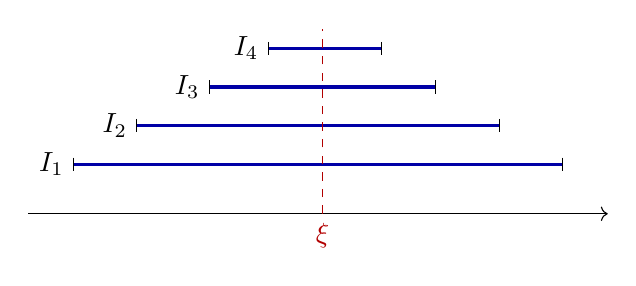
\begin{tikzpicture}[x=1.15cm,y=0.7cm]
  \draw[->] (-0.2,0) -- (6.2,0);
  \foreach \y/\a/\b/\lab in {0.9/0.3/5.7/I_1,1.6/1.0/5.0/I_2,2.3/1.8/4.3/I_3,3.0/2.45/3.7/I_4}
  {
    \draw[very thick,blue!65!black] (\a,\y)--(\b,\y);
    \draw (\a,\y+0.12)--(\a,\y-0.12);
    \draw (\b,\y+0.12)--(\b,\y-0.12);
    \node[left] at (\a,\y) {$\lab$};
  }
  \draw[dashed,red!70!black] (3.05,0)--(3.05,3.35);
  \node[below,red!70!black] at (3.05,0) {$\xi$};
\end{tikzpicture}
\end{center}

% SOURCE-END U0085
}
\end{frame}
% FRAME-ID F100
\begin{frame}[t,fragile]{极限存在性定理}
\footnotesize
{\footnotesize
% SOURCE-BEGIN U0086 0 85


下面的证明反复把一个有界区间二等分，并选择含有数列无穷多项的半区间。闭区间套性质保证这些不断缩小的闭区间最终确定一个实数点，这个点将成为所构造子列的极限。


% SOURCE-END U0086
}
\end{frame}
% FRAME-ID F101
\begin{frame}[t,fragile]{极限存在性定理}
\footnotesize
\begin{block}{定理}
{\footnotesize
% SOURCE-BEGIN U0087 0 74

\textbf{（有界数列必有收敛子列）}
任何有界数列 \(\{a_n\}\) 必定存在一个收敛的子列 \(\{a_{n_k}\}\)。

% SOURCE-END U0087
}
\end{block}
\end{frame}
% FRAME-ID F102
\begin{frame}[t,fragile]{极限存在性定理}
\footnotesize
{\footnotesize
% SOURCE-BEGIN U0088 0 735
\begin{custom}{证明}
设 $\{a_n\}$ 有界，则存在闭区间 $I_0=[\alpha_0,\beta_0]$ 包含数列的全部项。 将 $I_0$ 等分为左右两个闭区间。 至少有一个半区间包含数列中的无穷多项；否则两个半区间都只含有限多项，合起来也只含有限多项，与原数列有无穷多项矛盾。 取其中一个含无穷多项的半区间记为 $I_1$。

继续这个过程：把 $I_{k-1}$ 等分，取一个包含数列中无穷多项的半区间 $I_k$。 得到一列闭区间
\[
I_0\supset I_1\supset I_2\supset\cdots,\qquad |I_k|=\frac{|I_0|}{2^k}.
\]
根据闭区间套性质，存在唯一实数 $\xi$ 属于所有 $I_k$，并且区间长度趋于 $0$。

下面从数列中选子列。 因 $I_1$ 含无穷多项，可取 $n_1$ 使 $a_{n_1}\in I_1$。 取定 $n_1,\ldots,n_{k-1}$ 后，由于 $I_k$ 含无穷多项，可选 $n_k>n_{k-1}$ 使 $a_{n_k}\in I_k$。 于是得到子列 $\{a_{n_k}\}$。

任取 $\varepsilon>0$。 因 $|I_k|\to0$，存在 $K$，当 $k\ge K$ 时 $|I_k|<\varepsilon$。 对 $k\ge K$，$a_{n_k}$ 与 $\xi$ 同属 $I_k$，故
\[
|a_{n_k}-\xi|\le |I_k|<\varepsilon.
\]
由极限定义，$a_{n_k}\to\xi$。 因此有界数列必有收敛子列。
\end{custom}
% SOURCE-END U0088
}
\end{frame}
% FRAME-ID F103
\begin{frame}[t,fragile]{极限存在性定理}
\footnotesize
{\footnotesize
% SOURCE-BEGIN U0089 0 85
这个定理说的是：如果你有一列数，它们都挤在某个有限的区间里（比如都在 \([-M, M]\) 之间），那么无论它们看起来多么杂乱无章，你总能从中挑出一个“收敛”的子序列。
% SOURCE-END U0089
}
\end{frame}
% FRAME-ID F104
\begin{frame}[t,fragile]{极限存在性定理（续1）}
\footnotesize
{\footnotesize
% SOURCE-BEGIN U0089 85 158


\textbf{一个生活中的比喻：}

想象一个无限大的体育馆里有无穷多个人，每个人手里拿着一个数字，所有数字都在 0 到 1 之间。
% SOURCE-END U0089
}
\end{frame}
% FRAME-ID F105
\begin{frame}[t,fragile]{极限存在性定理（续2）}
\footnotesize
{\footnotesize
% SOURCE-BEGIN U0089 158 184
你想找出一群人，他们手里的数字越来越接近某个固定值。
% SOURCE-END U0089
}
\end{frame}
% FRAME-ID F106
\begin{frame}[t,fragile]{极限存在性定理（续3）}
\footnotesize
{\footnotesize
% SOURCE-BEGIN U0089 184 217


博尔查诺--魏尔斯特拉斯定理保证：你一定能找到这样一群人！
% SOURCE-END U0089
}
\end{frame}
% FRAME-ID F107
\begin{frame}[t,fragile]{极限存在性定理（续4）}
\footnotesize
{\footnotesize
% SOURCE-BEGIN U0089 217 251
无论这些人怎么站队，你总能挑出一个子序列，它最终会稳定在某个数附近。
% SOURCE-END U0089
}
\end{frame}
% FRAME-ID F108
\begin{frame}[t,fragile]{极限存在性定理（续5）}
\footnotesize
{\footnotesize
% SOURCE-BEGIN U0089 251 337


\textbf{一个更直观的几何解释：}

把数列 \(\{a_n\}\) 想象成数轴上的无限个点，所有点都被关在区间 \([-M, M]\) 这个“笼子”里。
% SOURCE-END U0089
}
\end{frame}
% FRAME-ID F109
\begin{frame}[t,fragile]{极限存在性定理（续6）}
\footnotesize
{\footnotesize
% SOURCE-BEGIN U0089 337 1378


\begin{center}
\begin{tikzpicture}[scale=0.8]
\draw[thick, -{Stealth}] (-5,0) -- (5,0) node[right] {数轴};
\draw[thick] (-4,0.1) -- (-4,-0.1) node[below] {\(-M\)};
\draw[thick] (4,0.1) -- (4,-0.1) node[below] {\(M\)};
\draw[thick, red] (-4,0.2) -- (4,0.2) node[above] {笼子（有界区间）};

\foreach \x in {-3.2, -1.5, -0.8, 0.3, 1.2, 2.5, 3.7, -2.1, 0.9, 2.8, -0.2, 1.9, -2.9, 3.1} {
    \filldraw[blue] (\x,0) circle (2pt);
}
\end{tikzpicture}
\end{center}

\textbf{核心思想——二分法：}

你可以用“不断对半分割区间”的方法来构造这个收敛子列：

\begin{enumerate}
\item 一开始，所有点都在区间 \([a, b] = [-M, M]\) 里。
\item 把这个区间分成两半：左边 \([-M, 0]\) 和右边 \([0, M]\)。由于有无穷多个点，至少有一半包含无穷多个点。选择那一半作为新区间 \([a_1, b_1]\)。
\item 再把新区间对半分，同样，至少有一半包含无穷多个点。选择那一半作为 \([a_2, b_2]\)。
\item 如此无限继续下去，我们得到一列不断缩小的区间：
\[
[a, b] \supset [a_1, b_1] \supset [a_2, b_2] \supset \cdots
\]
\item 每次区间的长度减半：\(b_n - a_n = \dfrac{2M}{2^n} \to 0\)。
\item 从每个区间里选出一个数列中的点 \(a_{n_k}\)，这些点就构成了一个收敛的子列。这些点被“挤压”在越来越小的区间里，最终会收敛到区间的公共极限点 \(c\)。
\end{enumerate}

\textbf{一个具体的例子：}

考虑数列 \(a_n = \sin n\)。
% SOURCE-END U0089
}
\end{frame}
% FRAME-ID F110
\begin{frame}[t,fragile]{极限存在性定理（续7）}
\footnotesize
{\footnotesize
% SOURCE-BEGIN U0089 1378 1450
虽然 \(\sin n\) 在 \([-1, 1]\) 之间振荡，看起来毫无规律，但博尔查诺--魏尔斯特拉斯定理告诉我们：一定存在一个子列收敛。
% SOURCE-END U0089
}
\end{frame}
% FRAME-ID F111
\begin{frame}[t,fragile]{极限存在性定理（续8）}
\footnotesize
{\footnotesize
% SOURCE-BEGIN U0089 1450 1521
事实上，可以证明 \(\sin n\) 的子列可以收敛到 \([-1, 1]\) 中的任意值，但这个定理只保证“存在”，不告诉我们具体是哪个。
% SOURCE-END U0089
}
\end{frame}
% FRAME-ID F112
\begin{frame}[t,fragile]{极限存在性定理（续9）}
\footnotesize
{\footnotesize
% SOURCE-BEGIN U0089 1521 1525



% SOURCE-END U0089
}
\end{frame}
% FRAME-ID F113
\begin{frame}[t,fragile]{极限存在性定理}
\footnotesize
{\footnotesize
% SOURCE-BEGIN U0090 0 579
\begin{custom}{单调有界准则与博尔查诺--魏尔斯特拉斯定理}

这两个定理是实数完备性的不同表现形式，它们实际上是等价的（在实数系中可以互相推导）。

\begin{tabular}{|c|c|c|}
\hline
 & \textbf{单调有界准则} & \textbf{博尔查诺--魏尔斯特拉斯定理} \\
\hline
\textbf{条件} & 数列单调 + 有界 & 数列有界（不要求单调） \\
\hline
\textbf{结论} & 数列本身收敛 & 存在收敛子列 \\
\hline
\textbf{适用场景} & 单调数列 & 任意有界数列 \\
\hline
\textbf{直观比喻} & 向右走，前面有墙 & 笼子里的无限多只鸟 \\
\hline
\end{tabular}

\textbf{关系：}
\begin{itemize}
\item 在额外具有单调性的条件下，单调有界准则能够推出整个数列收敛，结论更具体。
\item 博尔查诺--魏尔斯特拉斯定理适用于任意有界数列，但只保证其中存在收敛子列。
\item 两个定理的条件和结论不同，不能脱离前提简单地说谁“更强”。它们都是实数完备性的表现形式。
\end{itemize}

\end{custom}
% SOURCE-END U0090
}
\end{frame}
% FRAME-ID F114
\begin{frame}[t,fragile]{极限存在性定理}
\footnotesize
{\footnotesize
% SOURCE-BEGIN U0091 0 21

\fi


\iffalse

% SOURCE-END U0091
}
\end{frame}
\section{拓展阅读：Landau 符号-小o与大O}
% FRAME-ID F115
\begin{frame}[t,fragile]{目录（1/2）}
\normalsize
{\color{black}\normalsize 1. 数学内容\par}\vspace{0.3em}
{\color{black}\normalsize 2. 数列的一般定义\par}\vspace{0.3em}
{\color{black}\normalsize 3. 拓展阅读：数列的应用\par}\vspace{0.3em}
{\color{black}\normalsize 4. 差分及其应用\par}\vspace{0.3em}
{\color{black}\normalsize 5. 从实数的完备性说起\par}\vspace{0.3em}
{\color{black}\normalsize 6. 实数的完备性简介\par}\vspace{0.3em}
{\color{black}\normalsize 7. 数列极限\par}\vspace{0.3em}
{\color{black}\normalsize 8. 收敛数列的基本性质\par}\vspace{0.3em}
{\color{black}\normalsize 9. 极限存在性定理\par}\vspace{0.3em}
{\color{blue}\normalsize 10. 拓展阅读：Landau 符号-小o与大O\par}\vspace{0.3em}
\end{frame}
% FRAME-ID F116
\begin{frame}[t,fragile]{目录（2/2）}
\normalsize
{\color{gray!40}\normalsize 11. 第2章课后习题\par}\vspace{0.3em}
{\color{gray!40}\normalsize 12. 第2章参考答案与提示\par}\vspace{0.3em}
\end{frame}
% FRAME-ID F117
\begin{frame}[t,fragile]{拓展阅读：Landau 符号-小o与大O}
\footnotesize
{\footnotesize
% SOURCE-BEGIN U0092 0 123


在分析无穷小量（或无穷大量）时，我们常常需要比较它们趋近于零（或无穷）的“速度”或“阶”。Landau 符号（小 \(o\) 和大 \(O\)）提供了一套简洁的语言来描述这种比较关系。

\textbf{小o记号：高阶无穷小}


% SOURCE-END U0092
}
\end{frame}
% FRAME-ID F118
\begin{frame}[t,fragile]{拓展阅读：Landau 符号-小o与大O}
\footnotesize
\begin{block}{定义}
{\footnotesize
% SOURCE-BEGIN U0093 0 221

设 \(b_n\neq0\) 对充分大的 \(n\) 成立。若
\[
\lim_{n\to\infty}\dfrac{a_n}{b_n}=0,
\]
则记作
\[
a_n = o(b_n) \quad (n \to \infty).
\]
当 \(a_n,b_n\to0\) 时，称 \(a_n\) 是比 \(b_n\) 高阶的无穷小；当两者的绝对值趋于无穷时，则表示 \(a_n\) 相对 \(b_n\) 增长更慢。

% SOURCE-END U0093
}
\end{block}
\end{frame}
% FRAME-ID F119
\begin{frame}[t,fragile]{拓展阅读：Landau 符号-小o与大O}
\footnotesize
{\footnotesize
% SOURCE-BEGIN U0094 0 322
\(a_n = o(b_n)\) 的意思是：\(a_n\) 比 \(b_n\) “小得多”，或者说 \(a_n\) 趋近于 0 的速度比 \(b_n\) 快得多。

例如：
\[
\dfrac{1}{n^2} = o\left(\dfrac{1}{n}\right) \quad (n \to \infty),
\]
因为 \(\dfrac{1/n^2}{1/n} = \dfrac{1}{n} \to 0\)。这表示 \(1/n^2\) 比 \(1/n\) 更快地趋于 0。

更常见的用法是 \(a_n = o(1)\)，这直接表示 \(a_n \to 0\)（因为 \(\dfrac{a_n}{1} \to 0\)）。

% SOURCE-END U0094
}
\end{frame}
% FRAME-ID F120
\begin{frame}[t,fragile]{拓展阅读：Landau 符号-小o与大O}
\footnotesize
\begin{block}{例题}
{\footnotesize
% SOURCE-BEGIN U0095 0 375

当 \(n \to \infty\) 时：
\begin{itemize}
\item \(\dfrac{1}{n^2} = o\left(\dfrac{1}{n}\right)\)
\item \(\dfrac{1}{n} = o(1)\)
\item \(\dfrac{\ln n}{n} = o(1)\)
\item \(n = o(n^2)\)
\end{itemize}

\begin{custom}{函数情形的预告}
函数在 \(x\to x_0\) 时的小 \(o\) 记号必须建立在函数极限定义之上，下一章将正式讨论。届时可用
\[
f(x)=g(x)+o\bigl(h(x)\bigr)
\]
表示 \(f(x)-g(x)\) 相对于 \(h(x)\) 是高阶无穷小。
\end{custom}

% SOURCE-END U0095
}
\end{block}
\end{frame}
% FRAME-ID F121
\begin{frame}[t,fragile]{拓展阅读：Landau 符号-小o与大O}
\footnotesize
{\footnotesize
% SOURCE-BEGIN U0096 0 28


\textbf{大O记号：同阶或更低阶}


% SOURCE-END U0096
}
\end{frame}
% FRAME-ID F122
\begin{frame}[t,fragile]{拓展阅读：Landau 符号-小o与大O}
\footnotesize
\begin{block}{定义}
{\footnotesize
% SOURCE-BEGIN U0097 0 228

设当 \(n\to\infty\) 时，存在常数 \(C>0\) 和正整数 \(N\)，使得当 \(n>N\) 时，
\[
|a_n| \leq C |b_n|,
\]
则称 \(a_n\) 的量级不超过 \(b_n\)，记作
\[
a_n = O(b_n) \quad (n \to \infty).
\]

特别地，若 \(a_n=O(1)\)，表示 \(\{a_n\}\) 是有界数列。函数情形将在正式建立函数极限之后给出。

% SOURCE-END U0097
}
\end{block}
\end{frame}
% FRAME-ID F123
\begin{frame}[t,fragile]{拓展阅读：Landau 符号-小o与大O}
\footnotesize
{\footnotesize
% SOURCE-BEGIN U0098 0 276
\(a_n = O(b_n)\) 的意思是：\(|a_n|\) 不超过 \(|b_n|\) 的某个常数倍。它描述的是“增长（或衰减）速度不超过”的关系。

与 \(o\) 的区别：
\begin{itemize}
\item \(a_n = o(b_n)\) 意味着 \(a_n\) 比 \(b_n\) \textbf{严格更快}地趋于 0（或更慢地趋于无穷），比值趋于 0。
\item \(a_n = O(b_n)\) 意味着 \(a_n\) 与 \(b_n\) 同阶或更低阶，比值有界但不一定趋于 0。
\end{itemize}

% SOURCE-END U0098
}
\end{frame}
% FRAME-ID F124
\begin{frame}[t,fragile]{拓展阅读：Landau 符号-小o与大O}
\footnotesize
\begin{block}{例题}
{\footnotesize
% SOURCE-BEGIN U0099 0 512

当 \(n \to \infty\) 时：
\begin{itemize}
\item \(3n^2 + 2n + 1 = O(n^2)\)（因为 \(\dfrac{3n^2+2n+1}{n^2} \to 3\)，有界）
\item \(n \sin n = O(n)\)（因为 \(|\sin n| \leq 1\)，所以 \(|n \sin n| \leq n\)）
\item \(\dfrac{1}{n} = O\left(\dfrac{1}{n^2}\right)\)？不对！因为 \(\dfrac{1/n}{1/n^2} = n \to \infty\)，无界，所以 \(\dfrac{1}{n}\) 不是 \(O(1/n^2)\)。实际上 \(1/n^2 = O(1/n)\) 才对。
\end{itemize}

\begin{custom}{记号说明}
\(o(b_n)\) 与 \(O(b_n)\) 都不是某个固定数列，而是满足相应渐近条件的一类数列。同一个公式中重复出现的 \(o(b_n)\) 或 \(O(b_n)\)，也不一定代表同一个具体余项。
\end{custom}

% SOURCE-END U0099
}
\end{block}
\end{frame}
% FRAME-ID F125
\begin{frame}[t,fragile]{拓展阅读：Landau 符号-小o与大O}
\footnotesize
{\footnotesize
% SOURCE-BEGIN U0100 0 28


\textbf{小o与大O的关系与区别}


% SOURCE-END U0100
}
\end{frame}
% FRAME-ID F126
\begin{frame}[t,fragile]{拓展阅读：Landau 符号-小o与大O}
\footnotesize
{\footnotesize
% SOURCE-BEGIN U0101 0 807
\begin{custom}{对比表格}
\begin{tabular}{|c|c|c|}
\hline
\textbf{记号} & \textbf{含义} & \textbf{极限表述} \\
\hline
\(a_n = o(b_n)\) & \(a_n\) 比 \(b_n\) 高阶（或低阶） & \(\lim\limits_{n \to \infty} \dfrac{a_n}{b_n} = 0\) \\
\hline
\(a_n = O(b_n)\) & \(|a_n|\) 不超过 \(|b_n|\) 的常数倍 & \(\left|\dfrac{a_n}{b_n}\right|\) 最终有界 \\
\hline
\(a_n \sim b_n\) & 渐近等价（若二者趋于零，也称等价无穷小） & \(\lim \dfrac{a_n}{b_n} = 1\) \\
\hline
\end{tabular}

\textbf{关系：}
\[
a_n=o(b_n)\quad\Longrightarrow\quad a_n=O(b_n).
\]
反过来一般不成立。例如，\(\sin n=O(1)\) 但 \(\sin n\neq o(1)\)，因为 \(\sin n\) 不趋于 \(0\)。

\textbf{包含关系图：}
\begin{center}
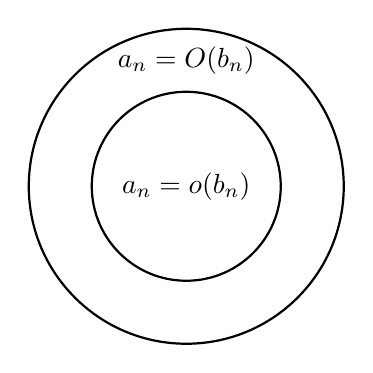
\begin{tikzpicture}
\draw[thick] (0,0) circle (2);
\draw[thick] (0,0) circle (1.2);
\node at (0,0) {$a_n = o(b_n)$};
\node at (0,1.6) {$a_n = O(b_n)$};
\end{tikzpicture}
\end{center}
\end{custom}
% SOURCE-END U0101
}
\end{frame}
% FRAME-ID F127
\begin{frame}[t,fragile]{拓展阅读：Landau 符号-小o与大O}
\footnotesize
{\footnotesize
% SOURCE-BEGIN U0102 0 111
\begin{custom}{无穷小与无穷大的关系}
若 \(\{a_n\}\) 是非零无穷小量，则 \(\left\{\dfrac{1}{a_n}\right\}\) 是无穷大量；反之亦然。
\end{custom}
% SOURCE-END U0102
}
\end{frame}
% FRAME-ID F128
\begin{frame}[t,fragile]{拓展阅读：Landau 符号-小o与大O}
\footnotesize
\begin{block}{例题}
{\footnotesize
% SOURCE-BEGIN U0103 0 376

当 \(n \to \infty\) 时：
\begin{itemize}
\item \(\dfrac{1}{n^p}\)（\(p>0\)）：\(p\) 越大，趋近 0 越快。
\item \(q^n\)（\(0 < q < 1\)）：指数衰减，比任何多项式都快。
\item \(\dfrac{1}{\ln n}\)：衰减极慢。
\item \(\dfrac{1}{n!}\)：衰减极快。
\end{itemize}

\textbf{增长率比较：} 当 \(n \to \infty\) 时，
\[
\ln n \ \ll\ n^p \ \ll\ a^n \ \ll\ n! \ \ll\ n^n \qquad (p>0,\ a>1).
\]
即：对数函数 < 幂函数 < 指数函数 < 阶乘 < \(n^n\)。

% SOURCE-END U0103
}
\end{block}
\end{frame}
% FRAME-ID F129
\begin{frame}[t,fragile]{拓展阅读：Landau 符号-小o与大O}
\footnotesize
{\footnotesize
% SOURCE-BEGIN U0104 0 444
\begin{application}[工程：温度传感器的迭代校准]
设 $T_n$ 为第 $n$ 次校准得到的温度估计，标准温度为 $T_{\mathrm s}$，单位均为 $^\circ\mathrm C$。假设每次校准保留上一估计误差的固定比例 $\alpha$，其中 $0<\alpha<1$：
\[
T_{n+1}=\alpha T_n+(1-\alpha)T_{\mathrm s}.
\]
于是
\[
T_{n+1}-T_{\mathrm s}=\alpha(T_n-T_{\mathrm s}),
\qquad
T_n-T_{\mathrm s}=\alpha^{n-1}(T_1-T_{\mathrm s}).
\]
由于 $\alpha^{n-1}\to0$，故 $T_n\to T_{\mathrm s}$。数列极限在这里描述“反复修正最终是否稳定”。模型假设校准比例固定，并忽略随机测量噪声与标准源漂移。
\end{application}
% SOURCE-END U0104
}
\end{frame}
% FRAME-ID F130
\begin{frame}[t,fragile]{拓展阅读：Landau 符号-小o与大O}
\footnotesize
{\footnotesize
% SOURCE-BEGIN U0105 0 195
农业中的谷物烘干也可出现相同的稳定结构。若第 $n$ 次观测的含水率满足
\[
M_n=M_{\mathrm e}+(M_0-M_{\mathrm e})q^n,\qquad0<q<1,
\]
则 $M_n\to M_{\mathrm e}$，其中 $M_{\mathrm e}$ 是给定环境下的平衡含水率。实际干燥速率会受温度、湿度、气流和谷层厚度影响，这里只作极限直观提示。

% SOURCE-END U0105
}
\end{frame}
% FRAME-ID F131
\begin{frame}[t,fragile]{拓展阅读：Landau 符号-小o与大O}
\footnotesize
{\footnotesize
% SOURCE-BEGIN U0106 0 11

\fi



% SOURCE-END U0106
}
\end{frame}
% FRAME-ID F132
\begin{frame}[t,fragile]{拓展阅读：Landau 符号-小o与大O}
\footnotesize
{\footnotesize
% SOURCE-BEGIN U0107 0 250
\begin{extra}
\subsection*{柯西收敛准则（选读）}

\begin{definition}[柯西列]
若对任意 \(\varepsilon > 0\)，存在 \(N\)，当 \(m,n > N\) 时 \(|a_m - a_n| < \varepsilon\)，则称 \(\{a_n\}\) 为柯西列。
\end{definition}
在实数集中，柯西列必收敛（这等价于实数的完备性）。柯西准则的好处是：判断收敛性时不需要知道极限值。
\end{extra}
% SOURCE-END U0107
}
\end{frame}
% FRAME-ID F133
\begin{frame}[t,fragile]{拓展阅读：Landau 符号-小o与大O}
\footnotesize
{\footnotesize
% SOURCE-BEGIN U0108 0 20



\iffalse



% SOURCE-END U0108
}
\end{frame}
\section{第2章课后习题}
% FRAME-ID F134
\begin{frame}[t,fragile]{目录（1/2）}
\normalsize
{\color{black}\normalsize 1. 数学内容\par}\vspace{0.3em}
{\color{black}\normalsize 2. 数列的一般定义\par}\vspace{0.3em}
{\color{black}\normalsize 3. 拓展阅读：数列的应用\par}\vspace{0.3em}
{\color{black}\normalsize 4. 差分及其应用\par}\vspace{0.3em}
{\color{black}\normalsize 5. 从实数的完备性说起\par}\vspace{0.3em}
{\color{black}\normalsize 6. 实数的完备性简介\par}\vspace{0.3em}
{\color{black}\normalsize 7. 数列极限\par}\vspace{0.3em}
{\color{black}\normalsize 8. 收敛数列的基本性质\par}\vspace{0.3em}
{\color{black}\normalsize 9. 极限存在性定理\par}\vspace{0.3em}
{\color{black}\normalsize 10. 拓展阅读：Landau 符号-小o与大O\par}\vspace{0.3em}
\end{frame}
% FRAME-ID F135
\begin{frame}[t,fragile]{目录（2/2）}
\normalsize
{\color{blue}\normalsize 11. 第2章课后习题\par}\vspace{0.3em}
{\color{gray!40}\normalsize 12. 第2章参考答案与提示\par}\vspace{0.3em}
\end{frame}
% FRAME-ID F136
\begin{frame}[t,fragile]{第2章课后习题}
\footnotesize
{\footnotesize
% SOURCE-BEGIN U0109 0 98

\addcontentsline{toc}{subsection}{第2章课后习题}

\subsubsection*{第2.1--2.5节\quad 数列的基本概念、表示与差分}


% SOURCE-END U0109
}
\end{frame}
% FRAME-ID F137
\begin{frame}[t,fragile]{第2章课后习题}
\footnotesize
{\footnotesize
% SOURCE-BEGIN U0110 0 301
写出下列数列的通项公式 \(a_n\)（用 \(n\) 表示）：
\begin{enumerate}
\item \(1, 3, 5, 7, 9, \dots\)
\item \(2, 4, 8, 16, 32, \dots\)
\item \(\dfrac{1}{2}, \dfrac{2}{3}, \dfrac{3}{4}, \dfrac{4}{5}, \dfrac{5}{6}, \dots\)
\item \(1, -\dfrac{1}{2}, \dfrac{1}{3}, -\dfrac{1}{4}, \dfrac{1}{5}, \dots\)
\end{enumerate}

% SOURCE-END U0110
}
\end{frame}
% FRAME-ID F138
\begin{frame}[t,fragile]{第2章课后习题}
\footnotesize
{\footnotesize
% SOURCE-BEGIN U0111 0 243
已知下列递推关系及初始条件，写出数列的前 5 项：
\begin{enumerate}
\item \(a_1 = 3\)，\(a_n = 2a_{n-1}\)（\(n \geq 2\)）
\item \(a_1 = 1\)，\(a_n = a_{n-1} + n\)（\(n \geq 2\)）
\item \(a_1 = 1\)，\(a_2 = 3\)，\(a_n = a_{n-1} - a_{n-2}\)（\(n \geq 3\)）
\end{enumerate}

% SOURCE-END U0111
}
\end{frame}
% FRAME-ID F139
\begin{frame}[t,fragile]{第2章课后习题}
\footnotesize
{\footnotesize
% SOURCE-BEGIN U0112 0 161
对于数列 \(a_n = n^2\)，计算：
\begin{enumerate}
\item 一阶差分 \(\Delta a_n\)
\item 二阶差分 \(\Delta^2 a_n\)
\item 三阶差分 \(\Delta^3 a_n\)
\end{enumerate}
观察结果，你能发现什么规律？

% SOURCE-END U0112
}
\end{frame}
% FRAME-ID F140
\begin{frame}[t,fragile]{第2章课后习题}
\footnotesize
{\footnotesize
% SOURCE-BEGIN U0113 0 259
求下列递推数列的通项公式：
\begin{enumerate}
\item \(a_1 = 1\)，\(a_n = a_{n-1} + 3\)（\(n \geq 2\)）
\item \(a_1 = 5\)，\(a_n = a_{n-1} + 2n - 1\)（\(n \geq 2\)）
\item \(a_1 = 2\)，\(a_n = 2a_{n-1} + 1\)（\(n \geq 2\)）\quad（提示：可设 \(b_n = a_n + 1\) 构造等比数列）
\end{enumerate}

% SOURCE-END U0113
}
\end{frame}
% FRAME-ID F141
\begin{frame}[t,fragile]{第2章课后习题}
\footnotesize
{\footnotesize
% SOURCE-BEGIN U0114 0 93
求一个数列 \(b_n\)，使得 \(\Delta b_n = n \cdot 2^n\)。
提示：设 \(b_n = (An + B)2^n\)，代入确定系数 \(A, B\)。

% SOURCE-END U0114
}
\end{frame}
% FRAME-ID F142
\begin{frame}[t,fragile]{第2章课后习题}
\footnotesize
{\footnotesize
% SOURCE-BEGIN U0115 0 109
用差分法求下列和式：
\begin{enumerate}
\item \(\sum_{k=1}^{n} k\)
\item \(\sum_{k=1}^{n} k(k+1)\)
\end{enumerate}

% SOURCE-END U0115
}
\end{frame}
% FRAME-ID F143
\begin{frame}[t,fragile]{第2章课后习题}
\footnotesize
{\footnotesize
% SOURCE-BEGIN U0116 0 283
已知斐波那契数列：\(F_1 = 1, F_2 = 1, F_n = F_{n-1} + F_{n-2} (n \geq 3)\)。
\begin{enumerate}
\item 计算比值 \(\dfrac{F_6}{F_5}, \dfrac{F_7}{F_6}, \dfrac{F_8}{F_7}, \dfrac{F_9}{F_8}, \dfrac{F_{10}}{F_9}\)，观察它们趋近于哪个数。
\item 证明：\(F_{n+1}F_{n-1} - F_n^2 = (-1)^n\)（卡西尼恒等式）。（选做）
\end{enumerate}

% SOURCE-END U0116
}
\end{frame}
% FRAME-ID F144
\begin{frame}[t,fragile]{第2章课后习题}
\footnotesize
{\footnotesize
% SOURCE-BEGIN U0117 0 201
已知数列 \(\{a_n\}\) 满足 \(a_1 = 1\)，且对任意 \(n \geq 1\) 有 \(\Delta a_n = 3^n\)。
\begin{enumerate}
\item 求 \(a_n\) 的通项公式。
\item 计算 \(\sum_{k=1}^{n} k \cdot 3^{k-1}\)。（提示：利用 \(a_n\) 的表达式）
\end{enumerate}

% SOURCE-END U0117
}
\end{frame}
% FRAME-ID F145
\begin{frame}[t,fragile]{第2章课后习题}
\footnotesize
{\footnotesize
% SOURCE-BEGIN U0118 0 185
已知一个数列的前几项为：\(a_1 = 1, a_2 = 5, a_3 = 14, a_4 = 30, a_5 = 55\)。
\begin{enumerate}
\item 计算该数列的一阶、二阶、三阶差分。
\item 根据差分结果判断 \(a_n\) 可能是几次多项式。
\item 求出 \(a_n\) 的通项公式。
\end{enumerate}

% SOURCE-END U0118
}
\end{frame}
% FRAME-ID F146
\begin{frame}[t,fragile]{第2章课后习题}
\footnotesize
{\footnotesize
% SOURCE-BEGIN U0119 0 250

设数列 \(\{a_n\}\) 满足 \(a_1 = 1\)，且 \(a_{n+1} = 3a_n + 2^n\)（\(n \geq 1\)）。
\begin{enumerate}
\item 令 \(b_n = \dfrac{a_n}{2^n}\)，写出 \(b_n\) 满足的递推关系。
\item 求 \(b_n\) 的通项公式。
\item 求 \(a_n\) 的通项公式。
\item 计算 \(\sum_{k=1}^{n} a_k\)。
\end{enumerate}

% SOURCE-END U0119
}
\end{frame}
% FRAME-ID F147
\begin{frame}[t,fragile]{第2章课后习题}
\footnotesize
{\footnotesize
% SOURCE-BEGIN U0120 0 54


\subsubsection*{第2.6--2.15节\quad 实数完备性与数列极限}



% SOURCE-END U0120
}
\end{frame}
% FRAME-ID F148
\begin{frame}[t,fragile]{第2章课后习题}
\footnotesize
{\footnotesize
% SOURCE-BEGIN U0121 0 246
用 \(\varepsilon\)-\(N\) 语言来说明这些数列的极限。
\begin{enumerate}
\item \(\lim\limits_{n\to\infty} \dfrac{3}{n} = 0\)
\item \(\lim\limits_{n\to\infty} \dfrac{1}{\sqrt{n}} = 0\)
\item \(\lim\limits_{n\to\infty} \dfrac{5n-2}{n+1} = 5\)
\end{enumerate}

% SOURCE-END U0121
}
\end{frame}
% FRAME-ID F149
\begin{frame}[t,fragile]{第2章课后习题}
\footnotesize
{\footnotesize
% SOURCE-BEGIN U0122 0 233
\begin{enumerate}
\item 如果数列 \(\{a_n\}\) 收敛，它的极限是否唯一？请简要说明理由。
\item 若 \(\lim\limits_{n\to\infty} a_n = 3\)，证明：存在正整数 \(N\)，使得当 \(n > N\) 时，\(a_n > 2\)。
\item 证明：若数列 \(\{a_n\}\) 收敛，则它必有界。（提示：取 \(\varepsilon = 1\)）
\end{enumerate}

% SOURCE-END U0122
}
\end{frame}
% FRAME-ID F150
\begin{frame}[t,fragile]{第2章课后习题}
\footnotesize
{\footnotesize
% SOURCE-BEGIN U0123 0 394
\begin{enumerate}
\item 判断下列数列是否为无穷小量：
   \[
   a_n = \dfrac{(-1)^n}{n},\quad b_n = \dfrac{n}{n+1},\quad c_n = 0.99^n,\quad d_n = \ln\left(1+\dfrac{1}{n}\right)
   \]
\item 判断下列数列是否为无穷大量：
   \[
   a_n = n^2,\quad b_n = (-1)^n n,\quad c_n = \ln n,\quad d_n = \dfrac{n^2}{n+1}
   \]
\item 若 \(\{a_n\}\) 是无穷小量且 \(a_n \neq 0\)，证明 \(\left\{\dfrac{1}{a_n}\right\}\) 是无穷大量。
\end{enumerate}

% SOURCE-END U0123
}
\end{frame}
% FRAME-ID F151
\begin{frame}[t,fragile]{第2章课后习题}
\footnotesize
{\footnotesize
% SOURCE-BEGIN U0124 0 250
用 \(\varepsilon\)-\(N\) 定义证明下列极限：
\begin{enumerate}
\item \(\lim\limits_{n\to\infty} \dfrac{\sin n}{n^2 + 1} = 0\)（提示：\(|\sin n| \leq 1\)）
\item \(\lim\limits_{n\to\infty} \dfrac{3n + \cos n}{2n - 1} = \dfrac{3}{2}\)（提示：先分拆，再放缩）
\end{enumerate}

% SOURCE-END U0124
}
\end{frame}
% FRAME-ID F152
\begin{frame}[t,fragile]{第2章课后习题}
\footnotesize
{\footnotesize
% SOURCE-BEGIN U0125 0 121
用 \(\varepsilon\)-\(N\) 定义证明：
\[
\lim_{n\to\infty} \left(\sqrt{n^2 + n} - n\right) = \dfrac{1}{2}.
\]
（提示：分子有理化后处理）

% SOURCE-END U0125
}
\end{frame}
% FRAME-ID F153
\begin{frame}[t,fragile]{第2章课后习题}
\footnotesize
{\footnotesize
% SOURCE-BEGIN U0126 0 140
设常数 \(c > 0\)，证明：
\[
\lim\limits_{n \to \infty} \dfrac{n^c}{a^n} = 0 \quad (a > 1).
\]
（提示：当 \(n\) 足够大时，\(a^n\) 增长快于任何幂函数；可用二项式定理或取对数）

% SOURCE-END U0126
}
\end{frame}
% FRAME-ID F154
\begin{frame}[t,fragile]{第2章课后习题}
\footnotesize
{\footnotesize
% SOURCE-BEGIN U0127 0 172
证明下列数列发散（极限不存在）：
\begin{enumerate}
\item \(a_n = (-1)^n\)
\item \(a_n = \sin\left(\dfrac{n\pi}{2}\right)\)
\item \(a_n = n + (-1)^n n\)（提示：考虑偶子列和奇子列）
\end{enumerate}

% SOURCE-END U0127
}
\end{frame}
% FRAME-ID F155
\begin{frame}[t,fragile]{第2章课后习题}
\footnotesize
{\footnotesize
% SOURCE-BEGIN U0128 0 151
用 \(\varepsilon\)-\(N\) 定义证明：
\[
\lim_{n\to\infty} \dfrac{n^2 - 2n + 3}{2n^2 + 5} = \dfrac{1}{2}.
\]
要求明确给出 \(N\) 关于 \(\varepsilon\) 的表达式（可分段处理）。

% SOURCE-END U0128
}
\end{frame}
% FRAME-ID F156
\begin{frame}[t,fragile]{第2章课后习题}
\footnotesize
{\footnotesize
% SOURCE-BEGIN U0129 0 296
用 \(\varepsilon\)-\(N\) 定义证明：
\begin{enumerate}
\item \(\lim\limits_{n\to\infty} \dfrac{\ln n}{n} = 0\)（提示：先证明当 \(n\) 充分大时 \(\ln n<\sqrt n\)，再取 \(N>\varepsilon^{-2}\)）
\item \(\lim\limits_{n\to\infty} \sqrt[n]{n} = 1\)（提示：设 \(\sqrt[n]{n} = 1 + h_n\)，利用二项式定理证明 \(h_n \to 0\)）
\end{enumerate}

% SOURCE-END U0129
}
\end{frame}
% FRAME-ID F157
\begin{frame}[t,fragile]{第2章课后习题}
\footnotesize
{\footnotesize
% SOURCE-BEGIN U0130 0 282
设 \(a_n = \dfrac{1}{n^2 + 1} + \dfrac{1}{n^2 + 2} + \cdots + \dfrac{1}{n^2 + n}\)。
\begin{enumerate}
\item 证明：\(\dfrac{n}{n^2 + n} \leq a_n \leq \dfrac{n}{n^2 + 1}\)。
\item 利用夹逼准则求 \(\lim\limits_{n\to\infty} a_n\)。
\item 用 \(\varepsilon\)-\(N\) 定义直接证明该极限。（选做）
\end{enumerate}

% SOURCE-END U0130
}
\end{frame}
% FRAME-ID F158
\begin{frame}[t,fragile]{第2章课后习题}
\footnotesize
{\footnotesize
% SOURCE-BEGIN U0131 0 295

设数列 \(\{a_n\}\) 满足：对任意 \(n\)，有 \(|a_{n+1} - a_n| \leq \dfrac{1}{2^n}\)。
\begin{enumerate}
\item 证明：对任意 \(m > n\)，有 \(|a_m - a_n| \leq \dfrac{1}{2^{n-1}}\)。（提示：用三角不等式和等比数列求和）
\item 证明：\(\{a_n\}\) 是柯西列，从而收敛。
\item 若已知 \(a_1 = 1\)，能否求出 \(\lim\limits_{n\to\infty} a_n\)？为什么？
\end{enumerate}

% SOURCE-END U0131
}
\end{frame}
\section{第2章参考答案与提示}
% FRAME-ID F159
\begin{frame}[t,fragile]{目录（1/2）}
\normalsize
{\color{black}\normalsize 1. 数学内容\par}\vspace{0.3em}
{\color{black}\normalsize 2. 数列的一般定义\par}\vspace{0.3em}
{\color{black}\normalsize 3. 拓展阅读：数列的应用\par}\vspace{0.3em}
{\color{black}\normalsize 4. 差分及其应用\par}\vspace{0.3em}
{\color{black}\normalsize 5. 从实数的完备性说起\par}\vspace{0.3em}
{\color{black}\normalsize 6. 实数的完备性简介\par}\vspace{0.3em}
{\color{black}\normalsize 7. 数列极限\par}\vspace{0.3em}
{\color{black}\normalsize 8. 收敛数列的基本性质\par}\vspace{0.3em}
{\color{black}\normalsize 9. 极限存在性定理\par}\vspace{0.3em}
{\color{black}\normalsize 10. 拓展阅读：Landau 符号-小o与大O\par}\vspace{0.3em}
\end{frame}
% FRAME-ID F160
\begin{frame}[t,fragile]{目录（2/2）}
\normalsize
{\color{black}\normalsize 11. 第2章课后习题\par}\vspace{0.3em}
{\color{blue}\normalsize 12. 第2章参考答案与提示\par}\vspace{0.3em}
\end{frame}
% FRAME-ID F161
\begin{frame}[t,fragile]{第2章参考答案与提示}
\footnotesize
{\footnotesize
% SOURCE-BEGIN U0132 0 101

\addcontentsline{toc}{subsection}{第2章参考答案与提示}

\subsubsection*{第2.1--2.5节\quad 数列的基本概念、表示与差分}


% SOURCE-END U0132
}
\end{frame}
% FRAME-ID F162
\begin{frame}[t,fragile]{第2章参考答案与提示}
\footnotesize
{\footnotesize
% SOURCE-BEGIN U0133 0 957
\begin{enumerate}
\item[(1)] (a) \(a_n = 2n-1\)；(b) \(a_n = 2^n\)；(c) \(a_n = \dfrac{n}{n+1}\)；(d) \(a_n = (-1)^{n-1} \dfrac{1}{n}\)。
\item[(2)] (a) \(3, 6, 12, 24, 48\)；(b) \(1, 3, 6, 10, 15\)；(c) \(1, 3, 2, -1, -3\)。
\item[(3)] \(\Delta a_n = 2n+1\)，\(\Delta^2 a_n = 2\)，\(\Delta^3 a_n = 0\)；规律：\(n^2\) 的二阶差分为常数，三阶及更高阶为 0。
\item[(4)] (a) \(a_n = 3n-2\)；(b) \(a_n = n^2 + 4\)；(c) \(a_n = 2^{n+1} - 1\)。
\item[(5)] \(b_n=(n-2)2^n+C\)（\(C\) 为任意常数）。
\item[(6)] (a) \(\dfrac{n(n+1)}{2}\)；(b) \(\dfrac{n(n+1)(n+2)}{3}\)。
\item[(7)] 比值趋近于 \(\dfrac{1+\sqrt{5}}{2} \approx 1.618\)。
\item[(8)] (a) \(a_n = \dfrac{3^n - 1}{2}\)；(b) \(\sum_{k=1}^{n} k \cdot 3^{k-1} = \dfrac{(2n-1)3^n + 1}{4}\)。
\item[(9)] 三阶差分为常数 \(2\)，是三次多项式，\(a_n=\dfrac{n(n+1)(2n+1)}{6}\)。
\item[(10)] (a) \(b_{n+1}=\dfrac{3}{2}b_n+\dfrac{1}{2}\)；(b) \(b_n=\left(\dfrac{3}{2}\right)^n-1\)；(c) \(a_n=3^n-2^n\)；(d) \(\sum_{k=1}^{n} a_k=\dfrac{3^{n+1}-3}{2}-(2^{n+1}-2)\)。
\end{enumerate}
% SOURCE-END U0133
}
\end{frame}
% FRAME-ID F163
\begin{frame}[t,fragile]{第2章参考答案与提示}
\footnotesize
{\footnotesize
% SOURCE-BEGIN U0134 0 54


\subsubsection*{第2.6--2.15节\quad 实数完备性与数列极限}



% SOURCE-END U0134
}
\end{frame}
% FRAME-ID F164
\begin{frame}[t,fragile]{第2章参考答案与提示}
\footnotesize
{\footnotesize
% SOURCE-BEGIN U0135 0 2051
\begin{enumerate}
\item[(1)] 
   (a) \(N = \lceil 3/\varepsilon \rceil\)；(b) \(N = \lceil 1/\varepsilon^2 \rceil\)；(c) \(\left|\dfrac{5n-2}{n+1} - 5\right| = \dfrac{7}{n+1}\)，取 \(N = \lceil 7/\varepsilon \rceil\)。

\item[(2)] 
   (a) 唯一，反证法用 \(\varepsilon = |L_1 - L_2|/2\) 导出矛盾；(b) 取 \(\varepsilon = 1\)，存在 \(N\) 使 \(n > N\) 时 \(|a_n-3|<1\)，故 \(a_n > 2\)；(c) 取 \(\varepsilon=1\)，有界性证明略。

\item[(3)] 
   (a) 无穷小量：\(a_n, c_n, d_n\)（\(b_n \to 1\) 不是）；(b) 无穷大量：\(a_n,b_n,c_n,d_n\)。其中 \(b_n=(-1)^n n\) 满足 \(|b_n|=n\to\infty\)，但 \(b_n\) 本身既不趋于 \(+\infty\)，也不趋于 \(-\infty\)；(c) 由定义直接验证。

\item[(4)] 
   (a) \(\left|\dfrac{\sin n}{n^2+1}\right| \leq \dfrac{1}{n^2}\)，取 \(N = \lceil 1/\sqrt{\varepsilon} \rceil\)；(b)
   \[
   \frac{3n+\cos n}{2n-1}-\frac32
   =\frac{2\cos n+3}{2(2n-1)},
   \]
   再利用 \(|2\cos n+3|\leq5\) 放缩。

\item[(5)] 
   分子有理化：\(\sqrt{n^2+n} - n = \dfrac{n}{\sqrt{n^2+n}+n} = \dfrac{1}{\sqrt{1+1/n}+1}\)，然后放缩证明。

\item[(6)] 
   取整数 \(m>c\)。当 \(n\geq2m\) 时，由二项式定理，
   \[
   a^n=(1+a-1)^n\geq\binom{n}{m}(a-1)^m
   \geq\frac{(n/2)^m}{m!}(a-1)^m.
   \]
   因而 \(0\leq n^c/a^n\leq Cn^{c-m}\to0\)。

\item[(7)] 
   (a) 子列极限不同；(b) 子列 \(0,1,0,-1,\dots\) 不收敛；(c) \(a_n = n(1+(-1)^n)\)，偶数项 \(\to +\infty\)，奇数项为 0。

\item[(8)] 
   \(\left|\dfrac{n^2-2n+3}{2n^2+5} - \dfrac{1}{2}\right| = \dfrac{4n+1}{2(2n^2+5)} < \dfrac{4n+1}{4n^2} < \dfrac{5}{4n}\)（当 \(n \geq 1\)），取 \(N = \lceil 5/(4\varepsilon) \rceil\)。

\item[(9)] 
   (a) 对充分大的 \(n\)，有 \(\ln n\leq\sqrt n\)，故 \(0\leq \ln n/n\leq1/\sqrt n\to0\)；(b) 由 \(\sqrt[n]{n}=1+h_n\)，二项展开得 \(n=(1+h_n)^n\geq\binom{n}{2}h_n^2\)，故 \(h_n^2\leq\dfrac{2}{n-1}\to0\)。

\item[(10)] 
   (a) 左边放缩：每项 \(\geq \dfrac{1}{n^2+n}\)，共 \(n\) 项；右边放缩：每项 \(\leq \dfrac{1}{n^2+1}\)；(b) 夹逼得极限为 0；(c) 直接证明：\(0 \leq a_n \leq \dfrac{1}{n}\)，取 \(N = \lceil 1/\varepsilon \rceil\)。

\item[(11)] 
   (a) \(|a_m - a_n| \leq \sum_{k=n}^{m-1} |a_{k+1}-a_k| \leq \sum_{k=n}^{\infty} \dfrac{1}{2^k} = \dfrac{1}{2^{n-1}}\)；(b) 由 (a) 知 \(\{a_n\}\) 是柯西列，故收敛；(c) 不能，因为只知道差值大小，不知道具体值。
\end{enumerate}
% SOURCE-END U0135
}
\end{frame}
% FRAME-ID F165
\begin{frame}[t,fragile]{第2章参考答案与提示}
\footnotesize
{\footnotesize
% SOURCE-BEGIN U0136 0 23

\fi

\clearpage


% SOURCE-END U0136
}
\end{frame}
\end{document}
